\documentclass[12pt,a4paper]{article}
\usepackage[utf8]{inputenc}
\usepackage[ngerman]{babel}
\usepackage[left=2.5cm,right=2.5cm,top=3cm,bottom=2cm]{geometry}
\author{Pauline Speckmann}
\usepackage{graphicx}
\usepackage{booktabs}
\usepackage{adjustbox}

\usepackage{fancyhdr}
\pagestyle{fancy}
\fancyhf{}
\fancyhead[l]{Digitalisierung $-$ Zusammenfassung von Pauline Speckmann}
\fancyhead[r]{\thepage}


\begin{document}
%%%%%%%%%%%%%%%%%%%%%%%%%%%%%%%%%%%%%%%%%%%%%%%%%%%%%%%%%%%%%%%%%%%%%%%%%%%%%%%%%%%%%%%%%%%%%%%%%%%%%%%%%%%%%%%%%%%%%%%%%%%%%%%%%%%%%%
%%%% VL 1
%%%%%%%%%%%%%%%%%%%%%%%%%%%%%%%%%%%%%%%%%%%%%%%%%%%%%%%%%%%%%%%%%%%%%%%%%%%%%%%%%%%%%%%%%%%%%%%%%%%%%%%%%%%%%%%%%%%%%%%%%%%%%%%%%%%%%%
\section{Informationssysteme als Gestaltungsgegenstand der Digitalisierung}

\vspace{0.5cm}
\subsection{Digitalisierung} %%%%%%%%%%%%%%%%%%%%%%%%%%%%%%%%%%%%%%%%%%%%%%%%%%%%%%%%%%%%%%%%%%%%%%%%%%%%%%%%%%%%%%%%%%%%%%%%%%%%%%%%%

\begin{itemize}
    \item \textbf{Begrifflichkeiten}:
       \begin{itemize}
          \item \textbf{Digitization}: Digitalisierung von Daten \\
		          Die Umwandlung von analogen in digitale Produkte und Dienstleistungen
		    \item \textbf{Digitalization}: Digitalisierung der Wertschöpfung \\
		          Die Veränderung von Geschäftsprozessen durch digitale Technologien
		    \item \textbf{Digitale Transformation}: \\
		          Die Neuorganisation von Geschäftsmodellen und Industrien durch digitale Technologien
       \end{itemize}
    
    \item \textbf{Der Einfluss der Digitalisierung auf die Organisation (Auswahl)}:
       \begin{itemize}
		    \item Abnehmende Distanz zwischen IT und Realität
		    \item Moorsches Gesetz
		    \item Kapselung von Funktionalitäten
		    \item KI-Entwicklung 
		\end{itemize}
\end{itemize}


\subsection{Wirtschaftsinformatik} %%%%%%%%%%%%%%%%%%%%%%%%%%%%%%%%%%%%%%%%%%%%%%%%%%%%%%%%%%%%%%%%%%%%%%%%%%%%%%%%%%%%%%%%%%%%%%%%%%%

\begin{itemize}
   \item \textbf{Was ist Ziel der Wirtschaftsinformatik?}\\
         Die Gestaltung von sozial akzeptablen, technisch stabilen und ökonomisch nachhaltigen Informationssystemen.
   
   \item \textbf{Paradigmen der Wirtschaftsinformatik:}
   \begin{itemize}
      \item \textbf{Realwissenschaft}: \\
            Einsatz von Informationssystemen in Wirtschaft, Verwaltung und dem privaten Lebensumfeld\\
            Schwerpunkt: Untersuchung von Einflüssen von IS im Unternehmen\\
            $\rightarrow$ Forschungsgegenstand sind reale Sachverhalte
      \item \textbf{Formalwissenschaft}: \\
            Entwicklung und Anwendung formaler Beschreibungsverfahren und Theorien 
            (bspw. zur Reduzierung der Komplexität (Modellierung))\\
            $\rightarrow$ Abstrakte Inhalte als Forschungsgegenstand
      \item \textbf{Ingenieurwissenschaft}: \\
            Gestaltung betrieblicher Informationssysteme\\
            $\rightarrow$ Technik und Entwicklung dieser
   \end{itemize}
\end{itemize}
 

\subsection{Informationssysteme} %%%%%%%%%%%%%%%%%%%%%%%%%%%%%%%%%%%%%%%%%%%%%%%%%%%%%%%%%%%%%%%%%%%%%%%%%%%%%%%%%%%%%%%%%%%%%%%%%%%%%

\begin{itemize}
   \item \textbf{Definition}:\\
         Bei Informationssystemen handelt es sich um soziotechnische (Mensch-Maschine) Systeme, die menschliche und maschinelle Komponenten (Teilsysteme) umfassen, insbesondere einer Aufgabenerfüllungdienen und zum Ziel der optimalen Bereitstellung von Informationen, Koordination und Kommunikation nach wirtschaftlichen Kriterien eingesetzt werden.

   \item \textbf{Charakteristika}:
      \begin{itemize}
         \item besteht aus Menschen und/oder Maschinen
         \item erzeugt oder benutzt Informationen
         \item verbindet Akteure durch Kommunikationsbeziehungen miteinander
      \end{itemize}
         
   \item \textbf{Ziele der Informationssysteme}:
			\begin{itemize}
			    \item Planung, Steuerung und Kontrolle in der Organisation unterstützen
			    \item Geschäftsprozesse beschleunigen
			    \item Qualität und Service verbessern
			    \item Wettbewerbsvorteile generieren
			\end{itemize}
   
   \item \textbf{Zentrale Begriffe, Normen und Abgrenzungen}:
   \item[] 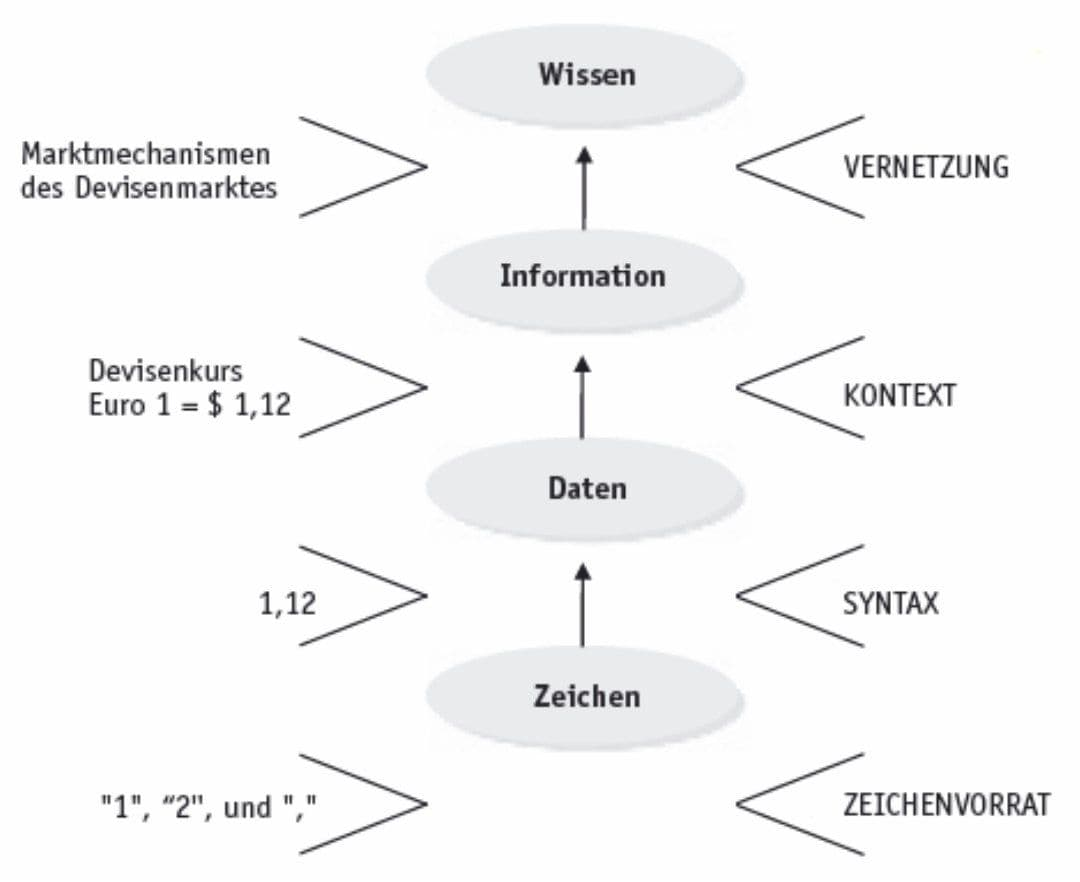
\includegraphics[scale=0.6]{ZentraleBegriffe-Normen-Abgrenzungen.jpg}

\newpage %Manuelle Formatierung
   \item \textbf{Teilsysteme in Unternehmen}:
         \begin{center}
            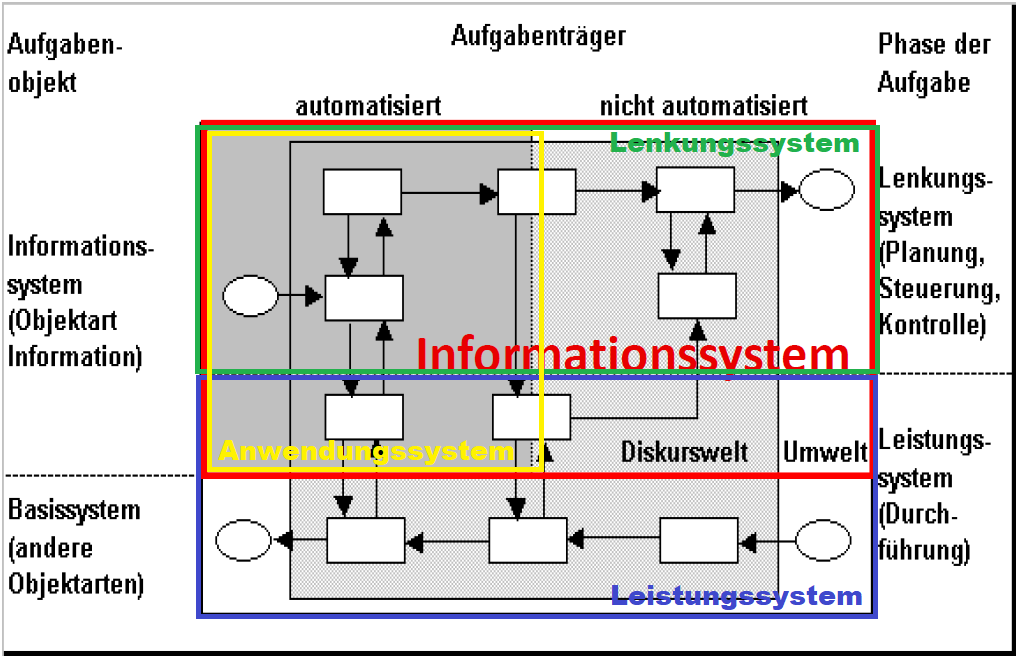
\includegraphics[scale=0.55]{Teilsysteme-in-Unternehmen.png}
         \end{center}
   
   \item \textbf{Ziele der Informationslogistik}:
         \begin{itemize}
            \item richtige Information (aktuell benötigt, verstanden, fehlerfrei)
            \item richtiger Zeitpunkt (Just in time (JIT))
            \item richtige Menge (so viel wie nötig, so wenig wie möglich)
            \item richtiger Ort (beim Empfänger verfügbar)
            \item erforderliche Qualität (ausreichend detailliert und wahr, unmittelbar verwendbar)
         \end{itemize}

   \item \textbf{Grundfragen bei der Gestaltung von Informationssystemen}:
      \begin{itemize}
         \item \textit{Wozu} (Auswertungszweck) wird die Information gebraucht?
         \item \textit{Wer} soll \textit{wen} über \textit{was} (Inhalt, Genauigkeit) informieren?
         \item \textit{Wann} (Termine) soll informiert werden?
         \item \textit{Wie} (Art, Form, Methode, Weg) soll informiert werden?
      \end{itemize}
\end{itemize}


\subsection{QUIZFRAGEN} %%%%%%%%%%%%%%%%%%%%%%%%%%%%%%%%%%%%%%%%%%%%%%%%%%%%%%%%%%%%%%%%%%%%%%%%%%%%%%%%%%%%%%%%%%%%%%%%%%%%%%%%%%%%%%
\begin{itemize}
   \item Der Schwerpunkt der Realwissenschaft als Paradigma der Wirtschaftsinformatik liegt in der Untersuchung von Einflüssen von Informationssystemen im Unternehmen.
   
   \item Ein Beispiel für die Informationsebene in der Begriffshierarchie ist \emph{die Note 1.3 eines Studenten im Fach Digitalisierung}, oder auch \emph{die Einordnung der Ziffernfolge '54785' als Matrikelnummer eines Studenten}.
   \item Um Daten in Informationen zu verwandeln, benötigt man eine Einordnung in einen bestimmten Kontext.
   
   \item Die Veränderung eines Vertriebskanals durch digitale Technologien wird durch die Terminologie \emph{Digitalization} beschrieben.
   \item Ein Beispiel für \emph{Digitale Transformation} ist: Durch das Corona Virus finden Lehrveranstaltungen nicht mehr physisch, sondern digital statt
   \item Dass früher Filme auf DVDs vertrieben wurden und heute per Stream abrufbar sind, fällt unter die \emph{Digitization}.
   
   \item Das Informationssystem eines Unternehmens umfasst sowohl automatisierte als auch nicht-automatisierte Aufgaben, aber nicht das Basissystem.
   
   \item Durch Informationssysteme werden die Ausprägungen Maschine-Mensch und Mensch-Mensch abgebildet.
   
   \item Das Ziel der Wirtschaftsinformatik ist die Gestaltung von sozial akzeptablen, technisch stabilen und ökonomisch nachhaltigen Informationssystemen.
   
   \item Häufig ändernde Kundenanforderungen als Eigenschaft der IT ermöglichen \emph{nicht} die Potenziale der Digitalisierung wie wir sie heute sehen.
   
   \item Eine Eigenschaft der Informationslogistik ist die Bereitstellung der Information am richtigen Ort.
\end{itemize}



%%%%%%%%%%%%%%%%%%%%%%%%%%%%%%%%%%%%%%%%%%%%%%%%%%%%%%%%%%%%%%%%%%%%%%%%%%%%%%%%%%%%%%%%%%%%%%%%%%%%%%%%%%%%%%%%%%%%%%%%%%%%%%%%%%%%%%
%%%% VL 2
%%%%%%%%%%%%%%%%%%%%%%%%%%%%%%%%%%%%%%%%%%%%%%%%%%%%%%%%%%%%%%%%%%%%%%%%%%%%%%%%%%%%%%%%%%%%%%%%%%%%%%%%%%%%%%%%%%%%%%%%%%%%%%%%%%%%%%
\newpage 
\section{Modellierung von Informationssystemen}

\vspace{0.5cm}
\subsection{Modellbegriff und Modellierung} %%%%%%%%%%%%%%%%%%%%%%%%%%%%%%%%%%%%%%%%%%%%%%%%%%%%%%%%%%%%%%%%%%%%%%%%%%%%%%%%%%%%%
\begin{itemize}
   \item Nutzen von Modellen
      \begin{itemize}
         \item \textbf{Grundzweck}: Reduktion von Komplexität
         \item Modell ist stets Modell mit Gegenstand (wovon), Zweck (wozu) und Zielgruppe (für wen)
      \end{itemize}
      
   \item Merkmale: Verkürzungs-, pragmatisches und Abbildungsmerkmal
   
   \item Realität $\rightarrow$ IST-Modell $\rightarrow$ SOLL-Modell
      \begin{itemize}
         \item \textbf{IST-Modell}:  Abbild der realen Welt
         \item \textbf{SOLL-Modell}: Zukünftige Möglichkeiten
      \end{itemize}

   \item \textbf{Geschäftsprozessmodellierung}:
      \begin{itemize}
         \item Erhöhung der Transparenz von Prozessen und Beziehungen innerhalb eines Unternehmens
         \item Erkennen von Zusammenhängen in betrieblichen Abläufen
         \item Erklärung der Funktionsweise des Unternehmens
         \item Erleichterung der Kommunikation im Unternehmen
         \item Grundlage zur Prozessoptimierung
         \item Einsatz zur Darstellung und Analyse verschiedener Lösungen
      \end{itemize}

   \item \textbf{Referenzmodell}:
      \begin{itemize}
         \item Immaterielle Abbildung der verarbeiteten Informationen
         \item Besitzt (im Gegensatz zu einem normalen Modell) normativen Charakter (Gestaltungsempfehlungen) und Heterogenität
         \item Allgemeingültigkeitsanspruch (Wahl einer adäquaten Abstraktion)
         \item Flexibilität: Veränderungen mit geringem Aufwand durchführen
      \end{itemize}
\end{itemize}


\subsection{Architektur integrierter Informationssysteme (ARIS)} %%%%%%%%%%%%%%%%%%%%%%%%%%%%%%%%%%%%%%%%%%%%%%%%%%%%%%%%%%%%%%%%
\begin{itemize}
   \item Architekturmodell zur Gestaltung einzelner Informationssysteme
          $\rightarrow$ Ausgangspunkt sind Vorgangskettenmodelle betrieblicher Bereiche
   \item ARIS umfasst:
      \begin{itemize}
        \item Vier Schichten: Daten (Zustände und Ereignisse), Funktionen, Steuerung und Organisation (inkludiert Bearbeiter)
        \item Drei Entwicklungsstufen
	        \begin{itemize}
	            \item[1)] Fachkonzept\\
	                  Ausgangspunkt für Umsetzung von Betriebswirtschaft in Informationstechnik
	                  (Anwendung einer formalisierten Sprache)
	            \item[2)] DV-Konzept (Datenverarbeitung)\\
	                  Übertragung der Begriffswelt von Fachkonzept in DV-Konzept und Definitionen
	            \item[3)] Implementierung\\
	                  Übergang des DV-Konzepts in Hard- und softwaretechnische Komponenten
	        \end{itemize}
      \end{itemize}
\end{itemize}


\subsection{Modellierung von Geschäftsprozessen} %%%%%%%%%%%%%%%%%%%%%%%%%%%%%%%%%%%%%%%%%%%%%%%%%%%%%%%%%%%%%%%%%%%%%%%%%%%%%%%%
\begin{itemize}
   \item \textbf{Ereignisgesteuerte Prozessketten (EPK)}:
       \begin{itemize}
		   \item Startereignis \& Endereignis
		   \item Modellierungselemente Ereignis \& Funktion
		   \item Operatoren AND, OR, XOR
		\end{itemize}
\end{itemize}

\vspace{-0.8cm}
\begin{center}
    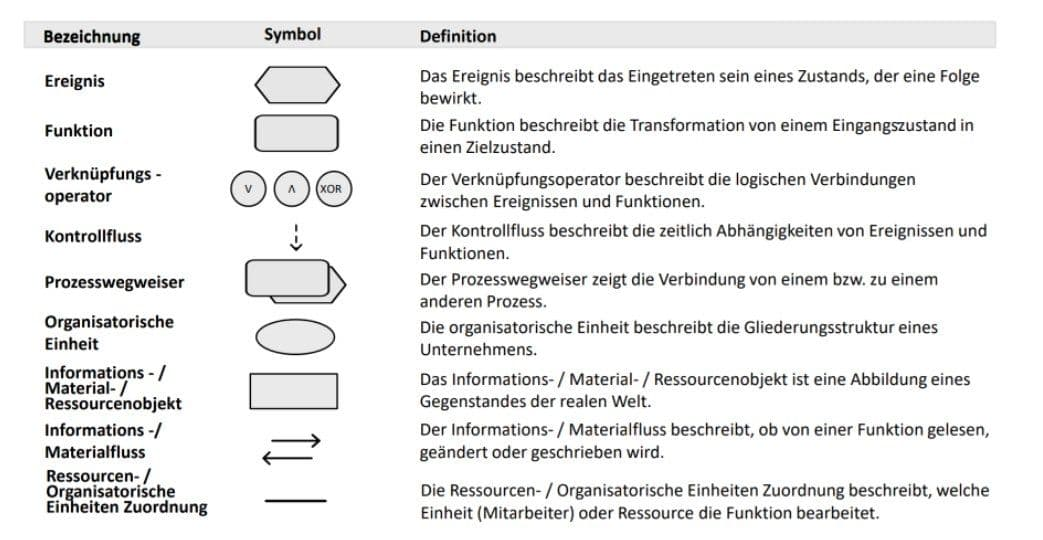
\includegraphics[width=1.05\textwidth]{digi2.jpg}
\end{center}

\begin{itemize}
\item []
   \begin{itemize}
      \item EPK braucht min. 1 Startereignis (oder Prozessschnittstelle)
	   \item EPK braucht min. 1 Endereignis (oder Prozessschnittstelle)
	   \item Auf Ereignis folgt Funktion oder Konnektor (Ausnahme: Endereignis)
	   \item Auf Funktion folgt Ereignis oder Konnektor
	   \item Jede Funktion hat genau eine ausgehende Kante
	   \item Jedes Ereignis hat genau eine eingehende und eine ausgehende Kante (Ausnahme: Start- und Endereignis)
	   \item Konnektor hat \textit{entweder} mehrere eingehende und genau eine ausgehende Kante 
	         \textit{oder} genau eine eingehende und mehrere ausgehende Kanten
   \end{itemize}
\end{itemize}


\subsection{Analyse von Geschäftsprozessen mit Process-Mining} %%%%%%%%%%%%%%%%%%%%%%%%%%%%%%%%%%%%%%%%%%%%%%%%%%%%%%%%%%%%%%%%%%
\begin{itemize}
   \item \textbf{$\alpha$-Algorithmus}:
      \begin{itemize}
         \item Grundidee:\\
               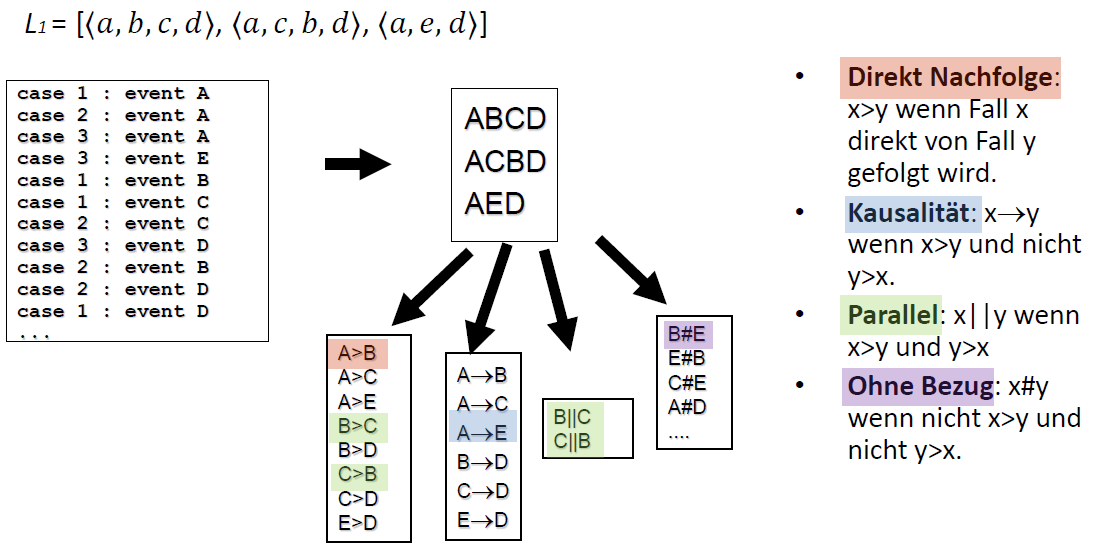
\includegraphics[width=0.9\textwidth]{alphaAlgorithmusGrundidee.png}
         \item Übersetzung ins finale Prozessmodell\\
               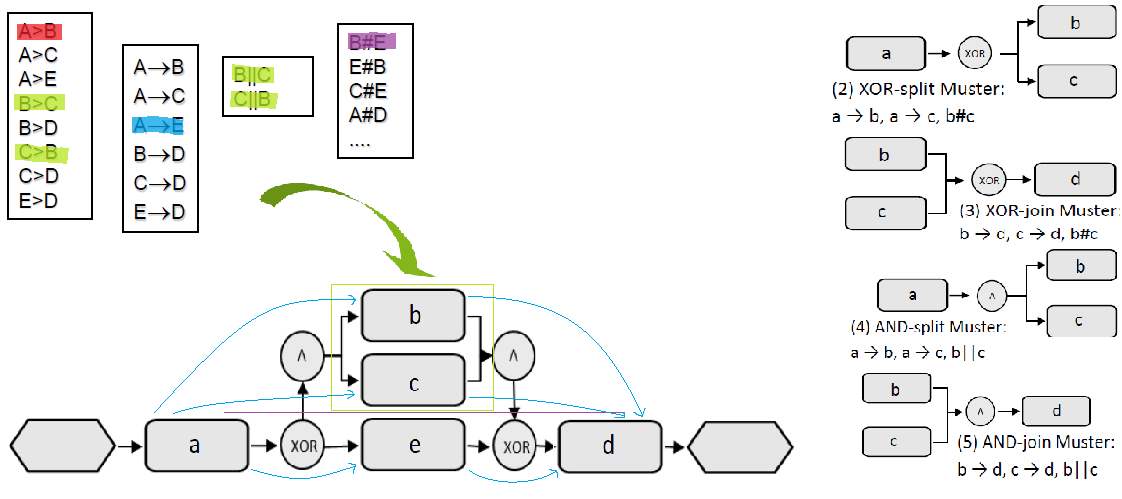
\includegraphics[width=0.9\textwidth]{alphaAlgFinalesModell.png}
      \end{itemize}
\end{itemize}


\vspace{0.5cm}
\subsection{QUIZFRAGEN} %%%%%%%%%%%%%%%%%%%%%%%%%%%%%%%%%%%%%%%%%%%%%%%%%%%%%%%%%%%%%%%%%%%%%%%%%%%%%%%%%%%%%%%%%%%%%%%%%%%%%%%%%%%%%%
\begin{itemize}
   \item Ein Ereignis in einem EPK beschreibt einen eingetretenen, für den Prozess relevanten, Zustand.
   \item Eine Funktion in einem EPK beschreibt eine fachliche Aufgabe oder Vorgang.
   
   \item Nutzen von Geschäftsprozessmodellierung sind die Verbesserung der organisationalen Kommunikation, die Steigerung der Effektivität von Prozessen und die Erhöhung der Transparnz von organissationalen Abläufen.
   
   \item Das Fachkonzept führt \emph{nicht} immer zum selben DV-Konzept.
   
   \item Die Gestaltungsempfehlung unterscheidet ein Referenzmodell von einem Modell.
   \item Modelle erfassen \emph{nicht} immer alle Individuen und Attribute des Originals
   \item Die Merkmale eines Modells sind das Pragmatische, das Abbildungs- und das Ver\-kürz\-ungs\-merk\-mal.
   
   \item Ein Beispiel für eine deduktive Vorgehensweise bei der Erstellung eines Referenzmodells ist \emph{die Erstellung eines Referenzmodells auf Basis einer Literaturrecherche oder wissenschaftlichen Theorien}.
\end{itemize}


%%%%%%%%%%%%%%%%%%%%%%%%%%%%%%%%%%%%%%%%%%%%%%%%%%%%%%%%%%%%%%%%%%%%%%%%%%%%%%%%%%%%%%%%%%%%%%%%%%%%%%%%%%%%%%%%%%%%%%%%%%%%%%%%%%%%%%
%%%% VL 3
%%%%%%%%%%%%%%%%%%%%%%%%%%%%%%%%%%%%%%%%%%%%%%%%%%%%%%%%%%%%%%%%%%%%%%%%%%%%%%%%%%%%%%%%%%%%%%%%%%%%%%%%%%%%%%%%%%%%%%%%%%%%%%%%%%%%%%
\newpage
\section{Management von Informationssystemen}

\vspace{0.5cm}
\subsection{Integrationsorientierte Informationssysteme} %%%%%%%%%%%%%%%%%%%%%%%%%%%%%%%%%%%%%%%%%%%%%%%%%%%%%%%%%%%%%%%%%%%%%%%%
\begin{itemize}
   \item \textbf{Digitaler Zwilling}:\\
         Digitale Darstellung eines realen Objekts oder Systems (materiell oder immateriell)

   \item \textbf{Integrationsansätze}
      \begin{itemize}
			\item \textbf{Datenintegration}:\\
			      Datenbestände von mehreren Informationssystemen werden zentral gespeichert (nicht mehrfach)
			\item \textbf{Funktionsintegration}:\\
			      Mehrere Funktionen werden in einem Informationssystem gebündelt
			\item \textbf{Prozess- oder Vorgangsintegration}:\\
			      In einem Prozess aufeinander folgende Funktionalitäten sind über ein Informationssystem nahtlos miteinander verbunden (Schnittstellen)
		\end{itemize}

   \item \textbf{SAP}: Global führender Anbieter von ERP-Systemen\\
         Beispiel: Verarbeitung eines Kundenauftrags
      \begin{enumerate}
			\item Kundenauftrag wird erfasst
			\item Automatisches Ausführen von: Bestellung der Rohmaterialien, Erzeugung von Fertigungsaufträgen, Übermittlung an die Finanzplanung
			\item Rollen \& Rechte verteilen
      \end{enumerate}

   \item \textbf{ERP- (Enterprise-Ressource-Planning) Systeme}:\\
         Integrierte betriebswirtschaftliche Softwarelösungen, die eine Vielzahl Ge\-schäfts\-pro\-zes\-se eines Unternehmens abdecken
      \begin{itemize}
			\item Hohe Datenintegration: Zentrale Datenbank
			\item Hohe Funktions- und Prozessintegration: Schnittstellen
      \end{itemize}
   \item[] 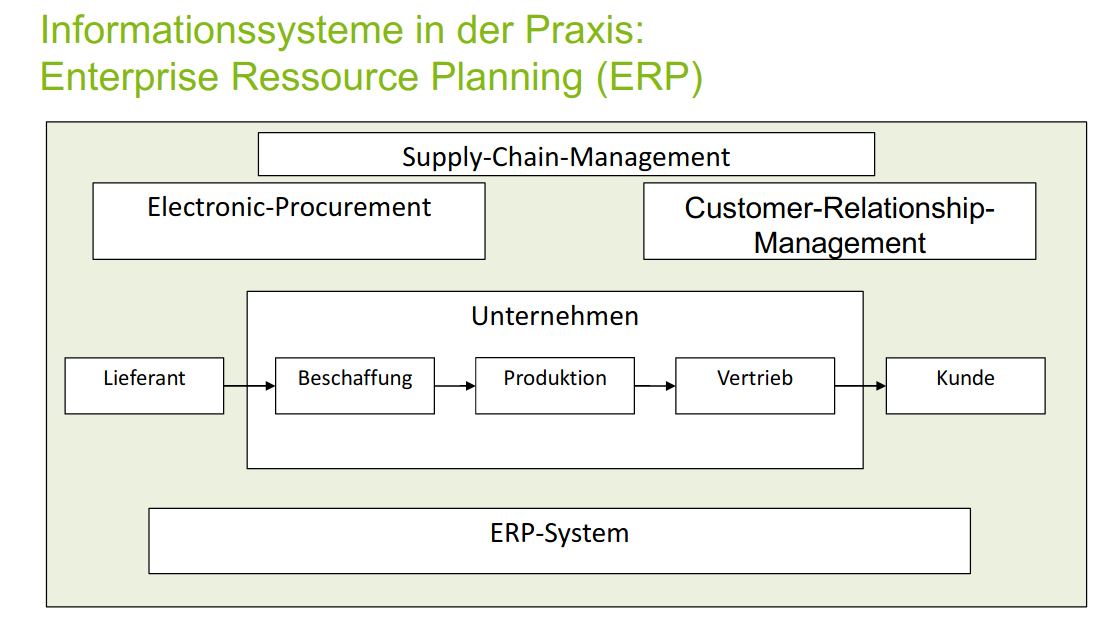
\includegraphics[scale=0.35]{digi_pic.png}
\end{itemize}


\subsection{Auswahl von Informationssystemen} %%%%%%%%%%%%%%%%%%%%%%%%%%%%%%%%%%%%%%%%%%%%%%%%%%%%%%%%%%%%%%%%%%%%%%%%%%%%%%%%%%%
\begin{itemize}
   \item \textbf{Systembereitstellung $–$ Goldene Regeln}:
   \item[] 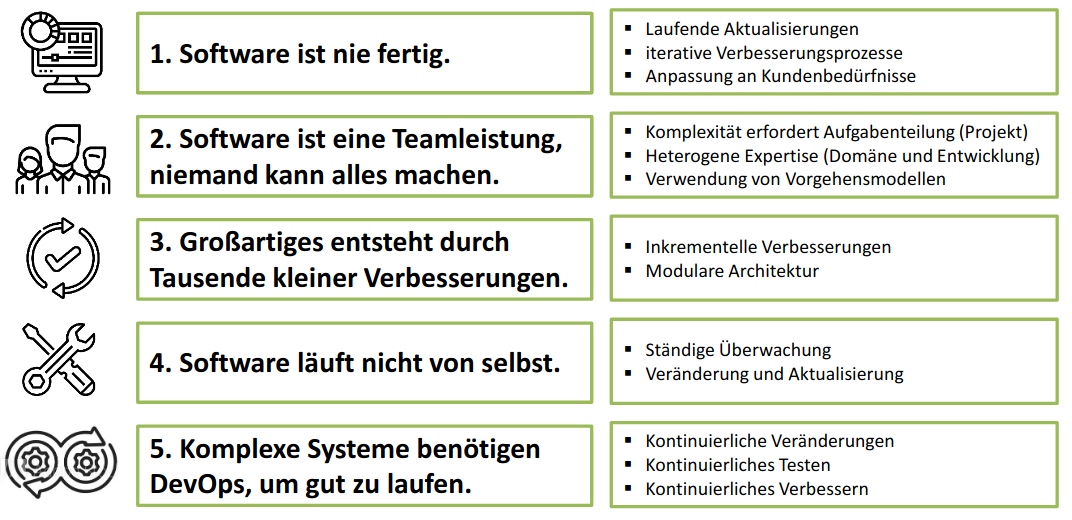
\includegraphics[scale=0.52]{GoldeneRegeln.png}
   
   \item \textbf{Softwareindustrie}:
      \begin{itemize}
			\item Direkte und Indirekte Netzeffekte:\\
			      Der Nutzen eines Programms für einen einzelnen Kunden steigt häufig mit der Gesamtzahl der Nutzer.
			\item Keine Vervielfältigungskosten:\\
			      Hohe initiale Entwicklungskosten, anschließend jedoch nahezu kostenfreie Ver\-viel\-fält\-ig\-ungs\-mög\-lich\-keit\-en (Fixkostendegression)
			\item Kein Wertverlust durch Gebrauch
			\item Make or buy?
         \item[] 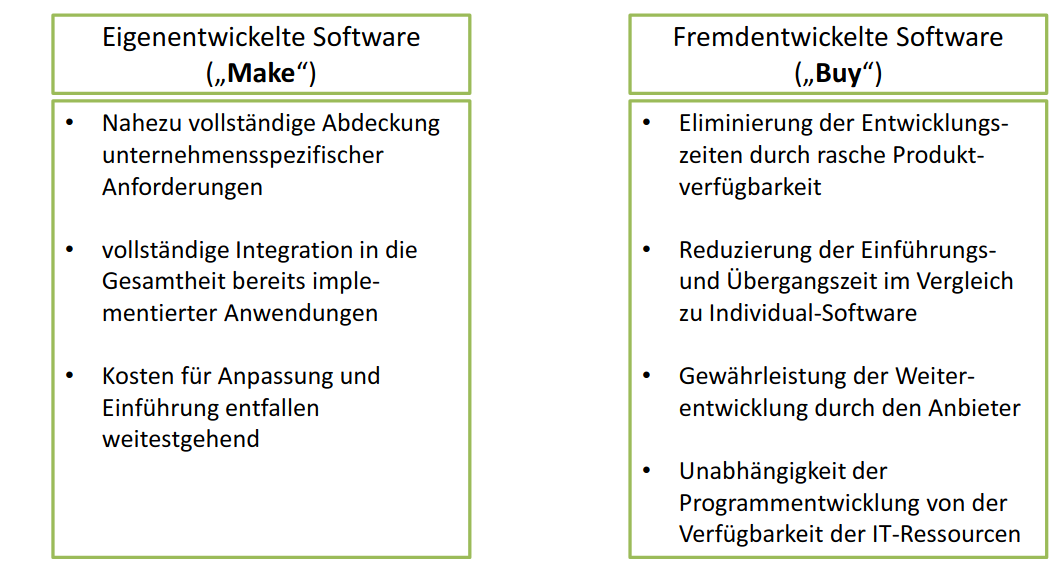
\includegraphics[scale=0.5]{MakeOrBuy.png}
%         \item[] \begin{minipage}[t]{0.43\textwidth} \vspace*{0cm}
%                     \begin{center}
%                        \textbf{Make}:\\
%                        Eigenentwickelte Software
%                     \end{center}
%                     \begin{itemize}
%                        \item Nahezu vollständige Abdeckung unternehmensspezifischer Anforderungen
%                        \item Vollständige Integration in die Gesamtheit bereits implementierter Anwendungen
%                        \item Kosten für Anpassung und Einführung entfallen weitestgehend
%                     \end{itemize}
%                  \end{minipage}
%                  \begin{minipage}[t]{0.45\textwidth} \vspace*{0cm}
%                     \begin{center}
%                        \textbf{Buy}:\\
%                        Fremdentwickelte Software
%                     \end{center}
%                     \begin{itemize}
%                        \item Eliminierung der Entwicklungszeiten durch rasche Produktverfügbarkeit
%                        \item Reduzierung der Einführungs- und Übergangszeit im Vergleich zu Individual-Software
%                        \item Gewährleistung der Weiterentwicklung durch den Anbieter
%                        \item Unabhängigkeit der Programmentwicklung von der Verfügbarkeit der IT-Ressourcen
%                     \end{itemize}
%                  \end{minipage}


\newpage %Manuelle Formatierung
         \item \textbf{Kostenvergleichsrechnung}:
         \item[] 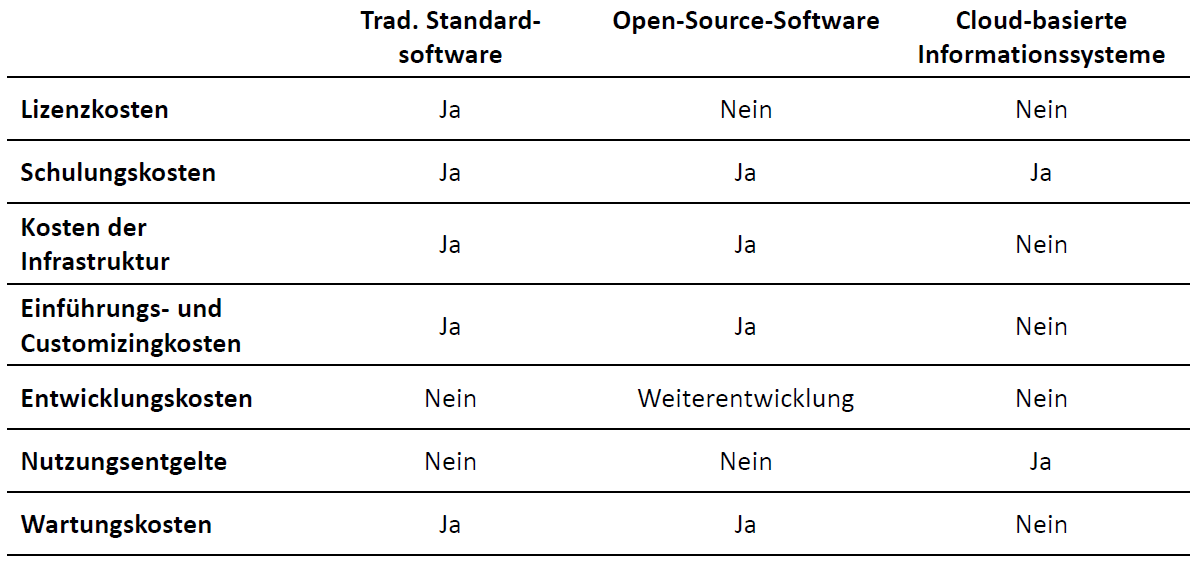
\includegraphics[scale=0.4]{Vergleichskosten.png}         
         
         \item \textbf{Nutzenkategorien von Informationssystemen}:
         \item[] 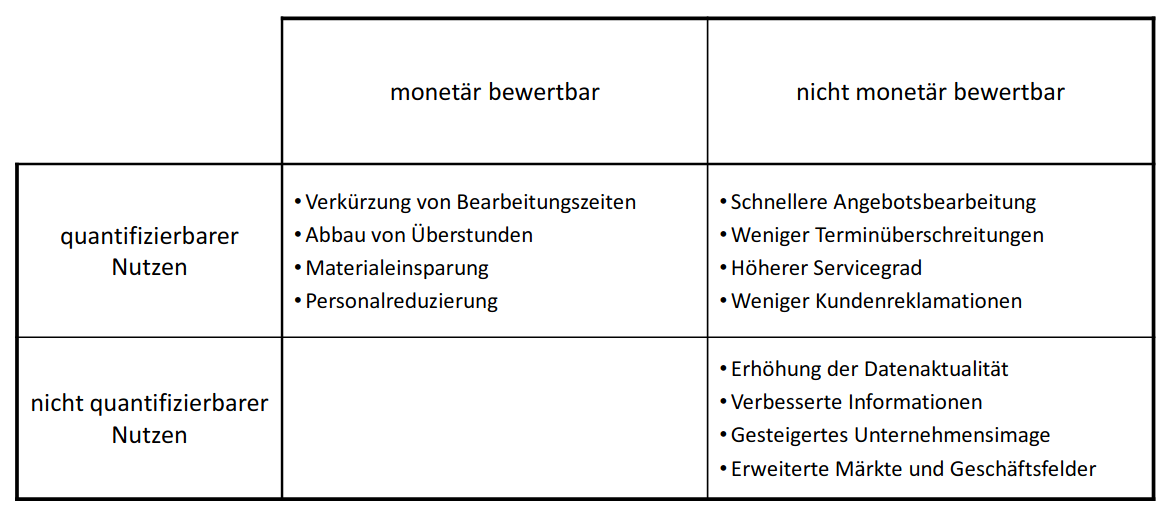
\includegraphics[scale=0.45]{Nutzen.png}
      \end{itemize}
   
   \item \textbf{Anwendungslebenszyklus}:\\
      \begin{minipage}[t]{0.3\textwidth}\vspace*{0cm}
         \begin{enumerate}
				\item Entwicklung
				\item Einführung
				\item Wachstum
				\item Sättigung / Reife
				\item Rückgang
				\item Abschaffung
         \end{enumerate}
      \end{minipage}
      \begin{minipage}[t]{0.3\textwidth}\vspace*{0cm}
         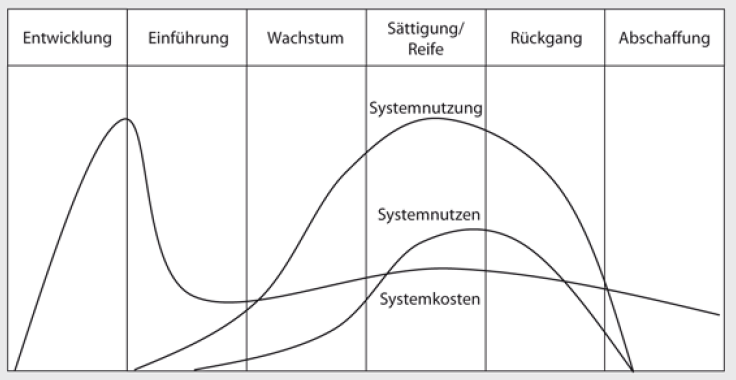
\includegraphics[scale=0.5]{Anwendungsleben.png}
      \end{minipage}
      
      
      
\end{itemize}


\subsection{Erstellung von Individualsoftware} %%%%%%%%%%%%%%%%%%%%%%%%%%%%%%%%%%%%%%%%%%%%%%%%%%%%%%%%%%%%%%%%%%%%%%%%%%%%%%%%%%
\begin{itemize}
   \item \textbf{Planung eines Softwareentwicklungsprozesses}:
      \begin{enumerate}
			\item Anforderungsanalyse und Erstellung einer Spezifikation
			\item Design
			\item Entwicklung
			\item Test und Integration
			\item Auslieferung des Produkts
			\item Wartung und Support
      \end{enumerate}
   
   \item \textbf{Strukturgetriebene Softwareentwicklung: Spiralmodell}\\
         Wiederholender Durchlauf von Entwicklungsphasen in Iterationen von jeweils 4 Schritten mit kontinuierlicher Bereitstellung von Prototypen.
      \begin{enumerate}
         \item \textbf{Analyse}:\\
                Definition von Rahmenbedingungen, Zielen, Anforderungen und Lö\-sungs\-alt\-er\-na\-ti\-ven, Freigabe zur Umsetzung
         \item \textbf{Evaluierung}:\\
                Evaluierung der umgesetzten Lösungsalternativen. Darauf basierend Erkennung von Risiken und Erarbeitung adäquater Strategien zur Vermeidung der Risiken.
         \item \textbf{Realisierung}:\\
                Definition und anschließende Realisierung des Vorgehens, basierend auf den identifizierten Risiken.
         \item \textbf{Planung}:\\
                Review der vorangegangenen Schritte und Planung der nächsten Iteration
      \end{enumerate}
   
   \item \textbf{Prinzipien agiler Softwareentwicklung}:
      \begin{itemize}
			\item Transparenz und Geschwindigkeit der Entwicklung erhöhen\\
			      Reaktion auf Änderungen $>$ Verfolgung eines festgelegten Plans
			\item Fehler minimieren\\
			      Funktionierende Software $>$ Umfangreiche Dokumentation
			\item Kommunikation und Interaktion!\\
			      Kooperation mit Projektbetroffenen $>$ Vertragsverhandlungen\\
			      Individuen und Interaktionen $>$ Prozesse und Tools
      \end{itemize}
   
   \item \textbf{SCRUM}:
      \begin{itemize}
			\item Modell der agilen Softwareentwicklung
			\item Transparenz, Überprüfung und Anpassung
			\item Grober, zeitlicher Rahmen wird definiert und dann angepasst\\
			      $\rightarrow$ Sprint Planning
			\item Teams sind selbstorganisiert\\
			      $\rightarrow$  Scrum Master, Product Owner, Team\\
			      $\rightarrow$ Daily SCRUM Meetings
      \end{itemize}
   
   \item \textbf{DevOps}:
      \begin{itemize}
			\item Development + Operations
			\item \textbf{Ziel}: In sich verändernden Umgebungen mit schlanken und flexiblen Software-Entwicklungsprozessen schnell zu reagieren
			\item DevOpszur Integration von Entwicklung und Betrieb:
			\item[] 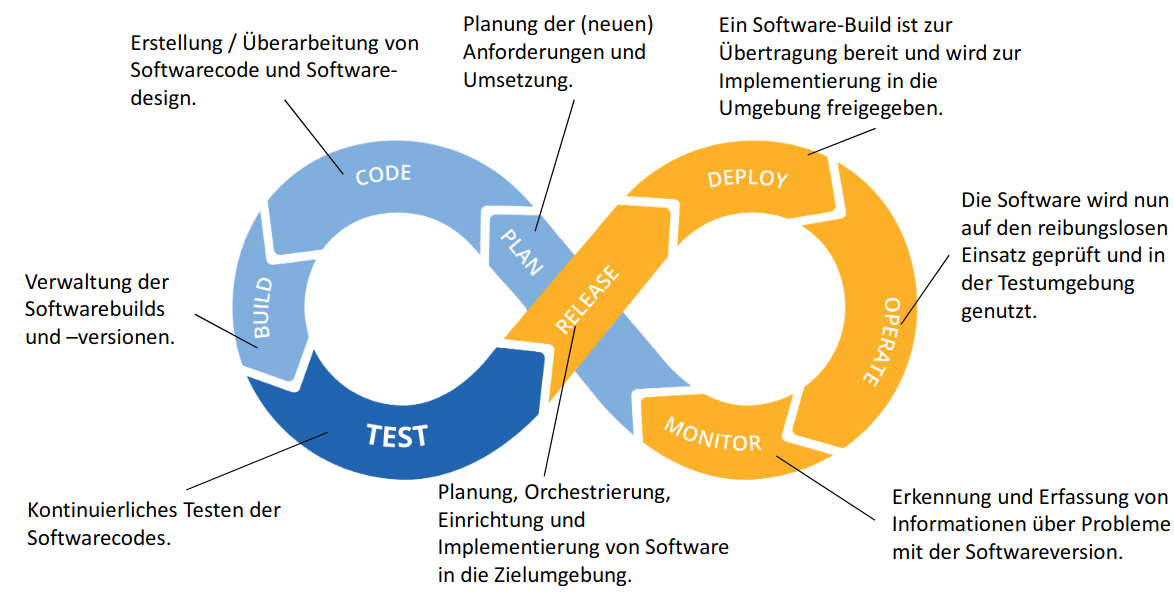
\includegraphics[scale=0.45]{DevOps.png}
			
			\item \textbf{Limitationen und Herausforderungen von DevOps}:
			   \begin{itemize}
					\item Flexibilität
					\item Automatisierung
					\item Lean-Prinzipien $\rightarrow$ System optimieren
					\item Alignment-Herausforderung $\rightarrow$ Überwachung der wichtigsten Indikatoren
					\item Kultur- und Wissensaustausch
            \end{itemize}
      \end{itemize}
   
   \item \emph{Magisches Dreieck} des Projektmanagements
   \item[] 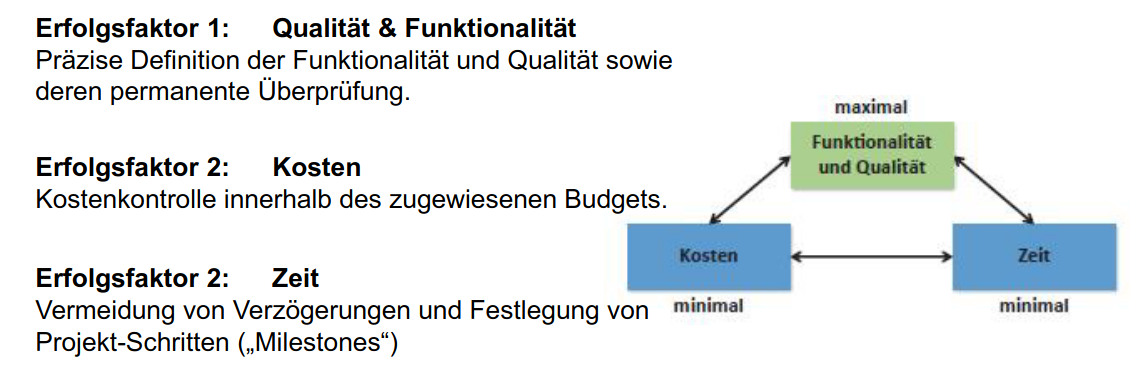
\includegraphics[scale=0.5]{magic.png}
\end{itemize}


\subsection{Beschaffung von Standardsoftware} %%%%%%%%%%%%%%%%%%%%%%%%%%%%%%%%%%%%%%%%%%%%%%%%%%%%%%%%%%%%%%%%%%%%%%%%%%%%%%%%%%%
\begin{itemize}
   \item \textbf{Vorgehen zur Softwareauswahl}:
      \begin{enumerate}
			\item Ist-Analyse
			\item Definition der Anforderung
			\item Marktanalyse
			\item Vergleich der Angebote
			\item Vertragsverhandlung
      \end{enumerate}
      
\newpage %Manuelle Formatierung
   \item \textbf{Kriterien für die Softwareauswahl}:
   \item[] 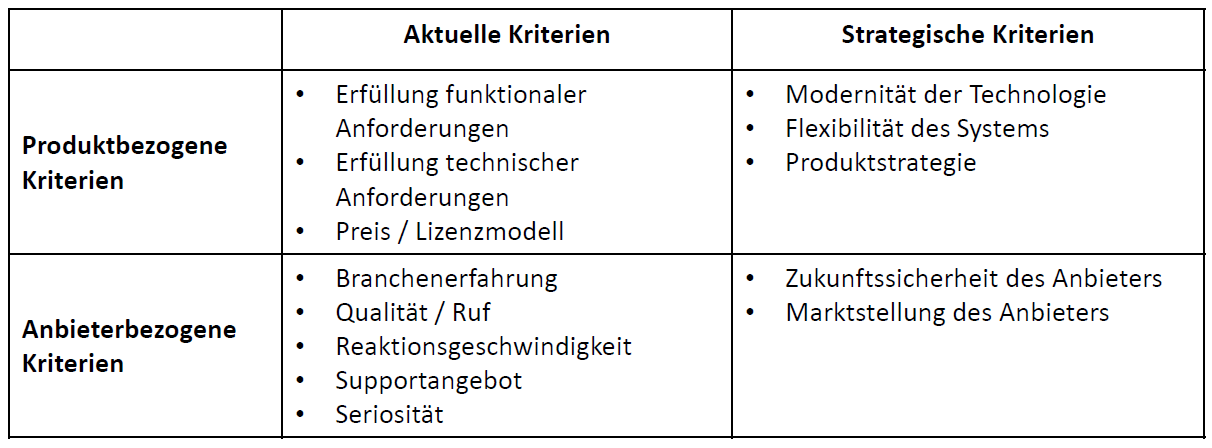
\includegraphics[scale=0.45]{KriterienSoftwareauswahl.png}
   
   \item \textbf{Proprietäre vs. Open Source Software}:
   \item[] 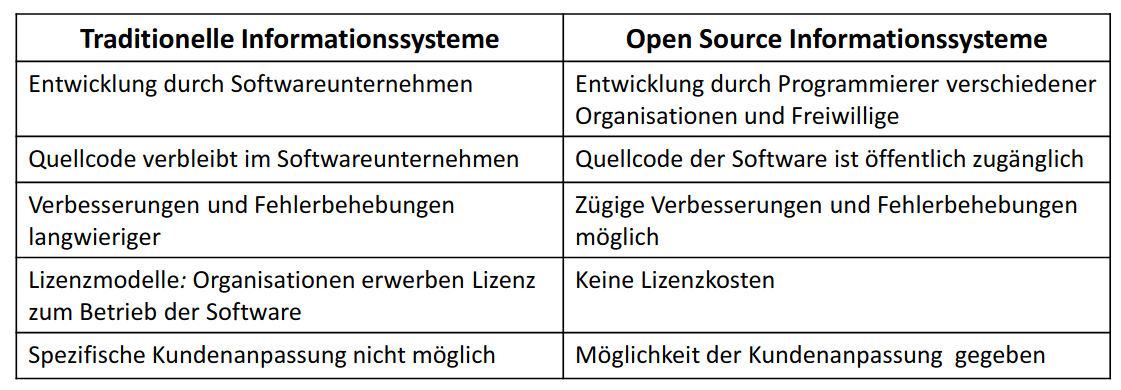
\includegraphics[scale=0.48]{foss.png}
   
   \item \textbf{IT-Outsourcing: Vor-und Nachteile}
   \item[] 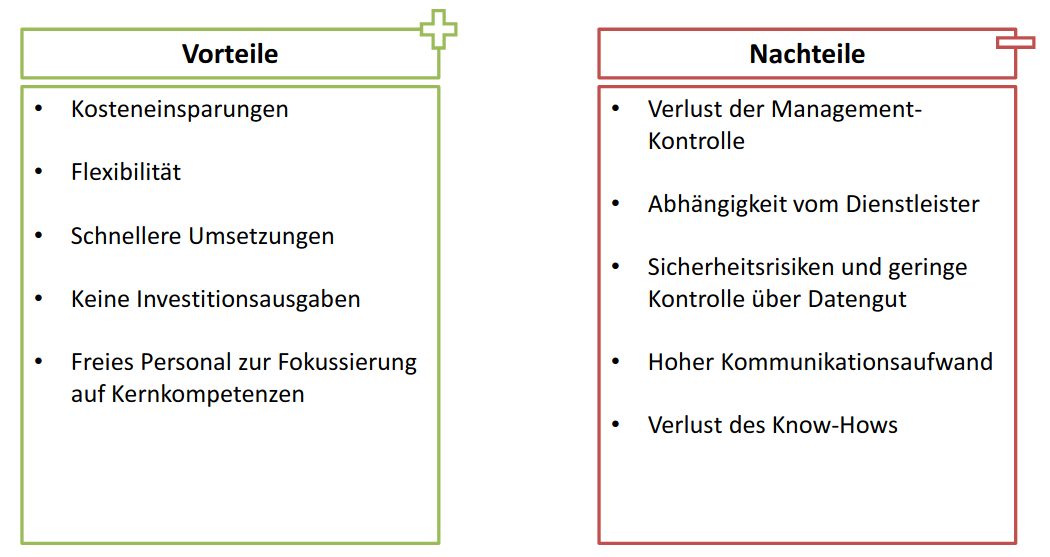
\includegraphics[scale=0.5]{out.png}
   
   \item \textbf{Cloud Computing}:\\
         Dynamische Bereitstellung von IT-Ressourcen über das Internet zur schnelleren Innovation und für flexiblere Ressourcen / Skaleneffekte
      \begin{itemize}
         \item \textbf{Infrastructure-as-a-Service (IaaS)}:\\
               Umfasst alle IT-Leistungen der Basisinfrastruktur z.B.Rechnerkapazitäten, Netzwerke und Speicherplatz.
         \item \textbf{Platform-as-a-Service (PaaS)}:\\
               IT-Leistungen, mit denen sich Anwendungssoftware und -komponenten entwickeln und integrieren lassen.
         \item \textbf{Software-as-a-Service (SaaS)}:\\
               Anwendungen und Dienste, die über Cloud Dienstebereitgestellt werden.
      \end{itemize}
\end{itemize}


\vspace{0.5cm}
\subsection{QUIZFRAGEN} %%%%%%%%%%%%%%%%%%%%%%%%%%%%%%%%%%%%%%%%%%%%%%%%%%%%%%%%%%%%%%%%%%%%%%%%%%%%%%%%%%%%%%%%%%%%%%%%%%%%%%%%%%%%%%
\begin{itemize}
   \item ERP-Systeme sind modular aufgebaut.
   
   \item Das Ziel der Prozess- oder Vorgangsintegration ist ursprünglich voneinander isolierte Prozesse aneinander anzugleichen oder auch zu verknüpfen.
   
   \item Vorteile von Standardsoftware (im Vergleich zu eigenentwickelter) sind die Ge\-währ\-leis\-tung der Programmwartung und -weiterentwicklung durch den Anbieter und der Profit vom \emph{Know-How}, das von vielen Anwendern in der Software abgebildet ist.
   
   \item  Bei Cloud Software werden Nutzungsentgelte verrechnet, aber es entstehen keine Wartungskosten für das nutzende Unternehmen.
   
   \item Die Zusammenarbeit verschiedenster Entwickler birgt ein immenses Innovationspotential bei Open Source Software.
   \item Bei Open Source Software kann der Quellcode von jedermann eingesehen, verändert, manipuliert und ausgebaut werden.
         Dabei gibt es weder Garantien noch einen klassischen Support.
         
   \item Wenn Unternehmen auf ein Höchstmaß an technischer und organisatorischer Integrität bestehen, sollten Sie die Software eigenstaendig entwickeln.
   \item Bei eigenetwickelter Software ist die Integration der Software unkompliziert, da die Software an die Prozesse angepasst wird.
   
   \item Agile Vorgehensmodelle haben eine gute Einsetzbarkeit bei unklaren Zielen und sich ändernden Anforderungen, erhöhten Kommunikations- und Abstimmungsaufwand, hohe Flexibilität und verringerte Komplexität der Projektverwaltung.
   
   \item SCRUM basiert auf der Grundannahme, dass eine detaillierte Planung zu Beginn wenig Sinn ergibt, da Projekte schlichtweg zu komplex sind.
   
   \item Cloud Computing unterscheidet sich vom IT-Outsourcing, indem lediglich einzelne Anwendungen ausgelagert werden, der Kern der IT aber im Unternehmen verbleibt.
\end{itemize}



%%%%%%%%%%%%%%%%%%%%%%%%%%%%%%%%%%%%%%%%%%%%%%%%%%%%%%%%%%%%%%%%%%%%%%%%%%%%%%%%%%%%%%%%%%%%%%%%%%%%%%%%%%%%%%%%%%%%%%%%%%%%%%%%%%%%%%
%%%% VL 4
%%%%%%%%%%%%%%%%%%%%%%%%%%%%%%%%%%%%%%%%%%%%%%%%%%%%%%%%%%%%%%%%%%%%%%%%%%%%%%%%%%%%%%%%%%%%%%%%%%%%%%%%%%%%%%%%%%%%%%%%%%%%%%%%%%%%%%
\newpage
\section{Konzept der digitalen Transformation}

\vspace*{0.5cm}
\subsection{Grundlagen digitale Transformation} %%%%%%%%%%%%%%%%%%%%%%%%%%%%%%%%%%%%%%%%%%%%%%%%%%%%%%%%%%%%%%%%%%%%%%%%%%%%%%%%%
\begin{itemize}
   \item \textbf{Potenziale von IT - Traditionelle Perspektive}
      \begin{itemize}
			\item Unstrukturierte Abläufe in routinemäßige Arbeit überführen
			\item Beschleunigung wertschöpfender Aktivitäten
			\item Ersatz und Reduktion menschlicher Arbeit
			\item Transport von Informationen mit großer Geschwindigkeit über große Entfernungen
			\item Große Menge von Informationen verfügbar machen
      \end{itemize}

   \item \textbf{Unternehmensstrategie und Informationssysteme}:
   \item[] 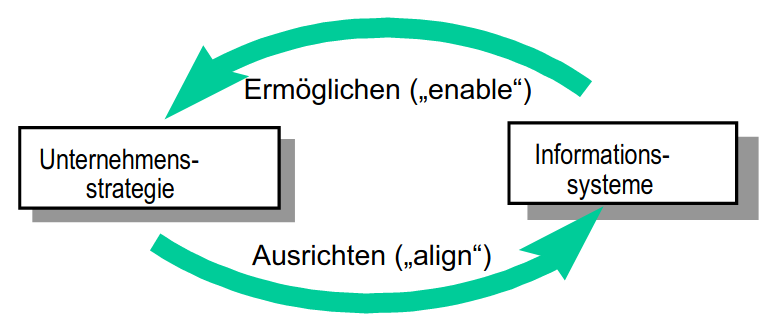
\includegraphics[scale=0.45]{UIS.png}
   
   \item \textbf{Potenziale digitaler Technologien für die Wertschöpfung}:
   \item[] 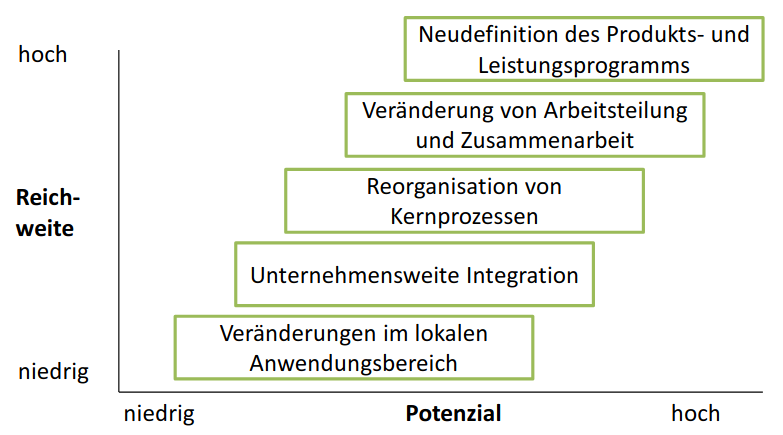
\includegraphics[scale=0.5]{Potenziale.png}
   
   \item \textbf{Digitale Transformation - Zentrale Schritte}:
      \begin{itemize}
			\item \textbf{Starke operationale Grundlage}: \\
			      Zuverlässige Kunden- und Produktdaten, End-to-End Transaktionsprozesse, Transparenz bei Kundentransaktionen
			\item \textbf{Experimentierfreudigkeit}: \\
			      Umfassende Einbindung von Mitarbeiter in Innovationsbemühungen
			\item \textbf{Datengesteuerte Entscheidungskultur}: \\
			      Hypothesenbildung, Datensammlung und detaillierte Auswertung, Top-Level Entscheidungskultur
			\item \textbf{Digitale Angebotsplattform}: \\
			      Wiederverwendbare Datentools und Algorithmen, Unterstützung bei der Konfiguration digitaler Lösungen
      \end{itemize}
\end{itemize}


\subsection{Digitale Technologie: Treiber der digitalen Transformation} %%%%%%%%%%%%%%%%%%%%%%%%%%%%%%%%%%%%%%%%%%%%%%%%%%%%%%%%%
\begin{itemize}
   \item Cloud Computing (Wiederholung von VL3)
   \item[] 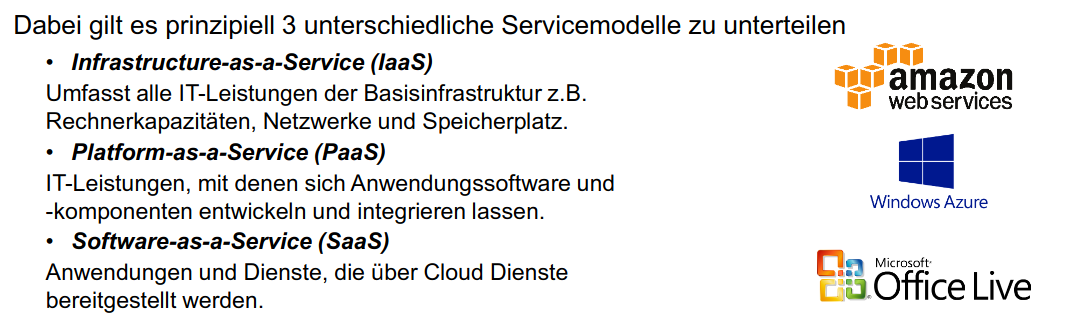
\includegraphics[scale=0.4]{repeat.png}
   \item[] \hspace*{0.5cm} 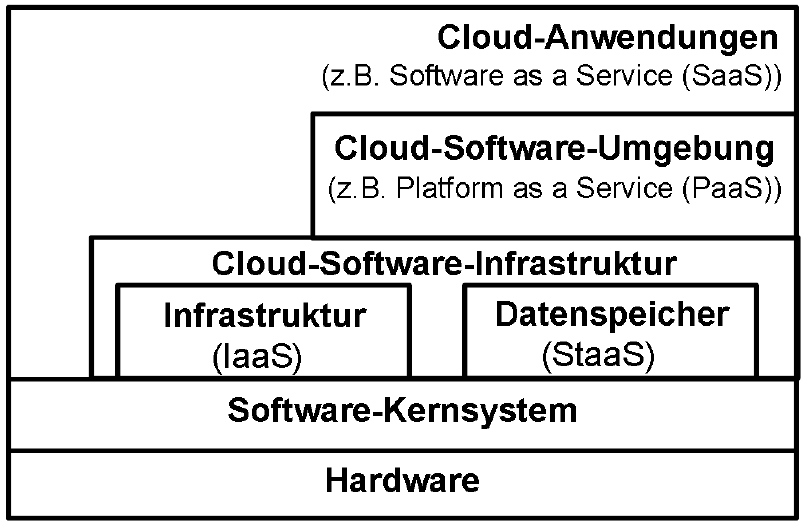
\includegraphics[scale=0.3]{CloudComputingKonzept.png}
   
   \item \textbf{Internet of Things}:\\
         Erweitertes Internet, in dem neben klassischen Rechnern und mobilen Endgeräten auch beliebige physische Gegenstände eingebunden werden

   \item \textbf{Augmented Reality}:
      \begin{itemize}
			\item Erweiterte Realität\\
			      Computergestützte Erweiterung der Realitätswahrnehmung
			\item Beispiel: mit App und Kamera Möbel virtuell in physischem Zimmer platzieren
      \end{itemize}

   \item \textbf{Blockchain}:
      \begin{itemize}
			\item Elektronisches Register (Liste) von Datensätzen (verteilte, öffentliche Datenbank)
			\item Dezentral verwaltet $\rightarrow$ sicher
			\item Blöcke (neue mit alten) werden unveränderbar miteinander verkettet
      \end{itemize}

   \item \textbf{Kerneigenschaften digitaler Technologien}:
      \begin{itemize}
			\item Homogenität der Daten:\\
			      Verschiedene Dateiformate können für verschiedene Zwecke genutzt werden
			\item Re-Programmierbarkeit:\\
			      Technologie kann für verschiedene Zwecke eingesetzt werden
			\item Selbstreferenzierung:\\
			      z.B. Kindle nutzt die Amazon Cloud zum Speichern der Bücher wodurch ab\-hän\-gi\-ge Netzwerkeffekte zu digitalen Innovation entstehen
      \end{itemize}
\end{itemize}


\subsection{Wertschöpfungsstrukturen verändern} %%%%%%%%%%%%%%%%%%%%%%%%%%%%%%%%%%%%%%%%%%%%%%%%%%%%%%%%%%%%%%%%%%%%%%%%%%%%%%%%%
\begin{itemize}
   \item \textbf{Veränderungen von Wertschöpfung durch digitale Transformation}:
   \item[] 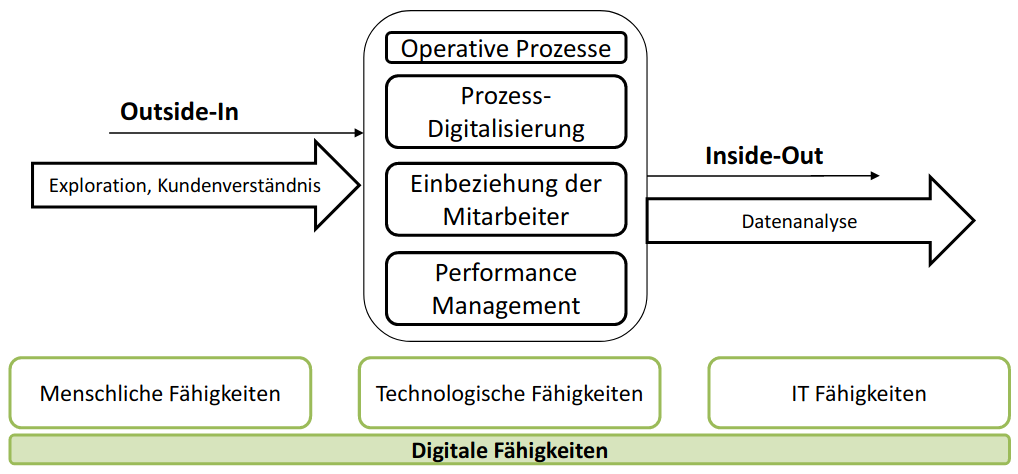
\includegraphics[scale=0.40]{veraenderung.png}
   
   \item \textbf{Digitale Fertigkeiten eines Unternehmens}:\\
         Digitale Daten und Informationstechnologien in seine Produkte, Dienstleistungen, Geschäftsprozesse und organisatorischen Systeme zu integrieren und so einen Mehrwert zu generieren
		\begin{itemize}
			\item IT-Unternehmenspartnerschaften
			\item Externe IT-Verbindungen
			\item Strategische Ausrichtung der IT
			\item IT Geschäftsprozessintegration
			\item IT Management
			\item IT Infrastruktur
		\end{itemize}

   \item \textbf{Wechselwirkung Produzent $–$ Konsument}:
   \item[] 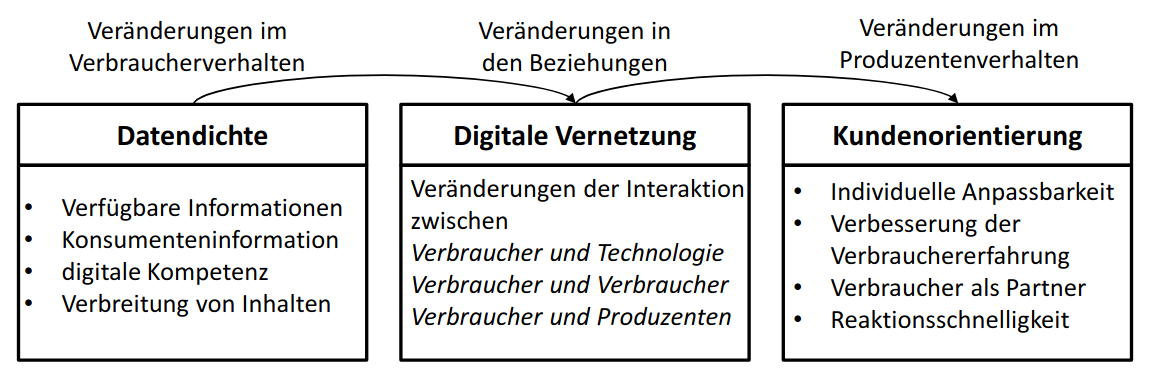
\includegraphics[scale=0.33]{prozess.png}
   
   \item \textbf{Modulare Architekturen}:\\
         Aufteilung eines Produktes in möglichst unabhängige Module (Verbund über standardisierte Schnittstellen)\\
         $\rightarrow$ Flexibilität
         
   \item \textbf{Consumerization}:
      \begin{itemize}
			\item Definition aus Vorlesung: \\
			Consumerization bezeichnet den spezifischen Einfluss, den verbraucherorientierte Technologien auf Unternehmen haben können. Sie spiegelt wider, wie Unternehmen von neuen Technologien und Modellen, die aus dem Konsumbereich und nicht aus dem Unternehmens-IT-Sektor stammen, beeinflusst werden und diese nutzen können.
			\item Wikipedia: \\
			Consumerization bezeichnet den Prozess bzw. die Erscheinung, dass elektronische Endgeräte, wie beispielsweise Smartphone, Tablet-PCs, von Arbeitnehmern auch für ihre Erwerbsarbeit benutzt werden.
      \end{itemize}
      

   \begin{minipage}[t]{0.4\textwidth}

	\textbf{Vorteile Consumerization} 
	\begin{itemize}
	\item bestimmte Arbeiten lassen sich dezentralisieren und flexibler organisieren und durchführen
	\item mehr Kontrolle der Arbeitnehmer über ihre Zeit und Arbeitsbeziehungen
	\end{itemize}

\end{minipage}\begin{minipage}[t]{0.1\textwidth}
   \ 
\end{minipage}\begin{minipage}[t]{0.4\textwidth}

	\textbf{Nachteile Consumerization} 
	\begin{itemize}
	\item auflösende Grenze zwischen Berufs- und Privatleben
	\item geringere Kontrollmöglichkeiten der Unternehmen
	\item Firmen können über die Netzwerkverbindungen auf die privat genutzten Geräte zugreifen
	\item Sicherheitsprobleme
	\end{itemize}


\end{minipage}
\end{itemize}

\vspace{0.5cm}
\subsection{QUIZFRAGEN} %%%%%%%%%%%%%%%%%%%%%%%%%%%%%%%%%%%%%%%%%%%%%%%%%%%%%%%%%%%%%%%%%%%%%%%%%%%%%%%%%%%%%%%%%%%%%%%%%%%%%%%%%%%%%%
\begin{itemize}
   \item Datenbasierte Verfahren sind auf dem Vormarsch.
   \item KI stellt eine neue Anforderung an die Widerstandsfähigkeit von Unternehmen gegen Fehler, was meint, dass:\\
         $\rightarrow$ Das KI-System ist nicht fehlerfrei. Dementsprechend muss das Unternehmen mit einer gewissen Anzahl an Fehlern rechnen/leben können.\\
         $\rightarrow$ Gerade bei neuen KI-Systemen werden Mitarbeiter Fehler in der Anwendung machen. Diese müssen einkalkuliert und toleriert werden.
   \item KI-Systementwicklungsprojekte unterscheiden sich von traditionellen Systementwicklungsprojekten durch eine intensivere initiale Auseinandersetzung mit der Unternehmenssituation, um eine passende KI-Lösung zu finden.
   \item Machine Learning gehört nicht zur schwachen KI Richtung.
   
   \item Software-as-a-Service (SaaS) hat die Vorteile der hohen Transparenz und Flexibilitaet bei den Kosten und der hohen Skalierbarkeit, da SaaS Zugänge schnell an den aktuellen Nutzerzahlen angepasst werden können.
   
   \item Mathematische Verfahren machen die Daten in der Blockchain zuverlässig und vertrauenswürdig und da die Datenbank verteilt ist, ist ein Ausfall des Netzwerks nahezu unmöglich.
   
   \item Ziel der digitalen Transformation ist es durch intensive Experimente neue Ge\-schäfts\-mo\-del\-le zu kreieren.
   
   \item Die Reprogrammierbarkeit als Kern-Eigenschaft einer digitaler Technologien bedeutet, dass verschiedene Funktionen von einem einzigen digitalen Gerät ausgeführt werden können.
   \item Durch die Reprogrammierbarkeit kann ein digitales Gerät eine Vielzahl von Funktionen ausführen (z.B. Textverarbeitung, Videobearbeitung und Web-Browsing).
   \item Die Selbst-Referenzierbarkeit als Kern-Eigenschaft einer digitaler Technologie bedeutet, dass digitale Innovation den Einsatz digitaler Technologien erfordern.
   \item Homogenisierung von Daten bedeutet, dass alle digitalen Inhalte mit den gleichen digitalen Geräten und Netzwerken gespeichert, übertragen, verarbeitet und angezeigt werden können.
   
   \item Das Internet der Dinge bezeichnet die Verbindung von Gegenständen mit dem Internet, damit diese Gegenstände selbstständig über das Internet kommunizieren können.
   
   \item Der Mensch spielt in der gegenseitigen Beeinflussung von Organisation und IT nur eine untergeordnete Rolle, denn der Zusammenhang zwischen Organisation und IT ist direkt.
   
   \item Die Implementierung voneinander getrennter Business- und IT-Abteilungen ist keine digitale Fähigkeit.
   
   \item Bestandteile der Definition von \emph{Digitale Transformation} sind die Auswirkungen auf Aspekte der Wirtschaft und der Gesellschaft und die Nutzung von Digitalen Innovationen.
\end{itemize}


%%%%%%%%%%%%%%%%%%%%%%%%%%%%%%%%%%%%%%%%%%%%%%%%%%%%%%%%%%%%%%%%%%%%%%%%%%%%%%%%%%%%%%%%%%%%%%%%%%%%%%%%%%%%%%%%%%%%%%%%%%%%%%%%%%%%%%
%%%% VL 5
%%%%%%%%%%%%%%%%%%%%%%%%%%%%%%%%%%%%%%%%%%%%%%%%%%%%%%%%%%%%%%%%%%%%%%%%%%%%%%%%%%%%%%%%%%%%%%%%%%%%%%%%%%%%%%%%%%%%%%%%%%%%%%%%%%%%%%
\newpage
\section{Management der digitalen Transformation}

\vspace*{0.5cm}
\subsection{Transformationsstrategien entwickeln} %%%%%%%%%%%%%%%%%%%%%%%%%%%%%%%%%%%%%%%%%%%%%%%%%%%%%%%%%%%%%%%%%%%%%%%%%%%%%%%%%

\begin{itemize}
   \item \textbf{Sichten auf Transformationsstratiegien}

   \item[] $\rightarrow$ \textbf{Innovationsperspektive:}
      \begin{itemize}
         \item Phase 1: Experimentieren am Rande der Organisation
               \begin{itemize}
                  \item Ergänzende Experimente: \\
                        Das bestehende Geschäftsmodell bleibt bestehen, Innovation beruht auf das vorhandene Geschäftsmodell.
                  \item Disruptive Experimente: \\
                        Das Geschäftsmodell wird grundlegend innoviert.
                  \item Von der Beobachtung zur Verpflichtung:
                  \item[] 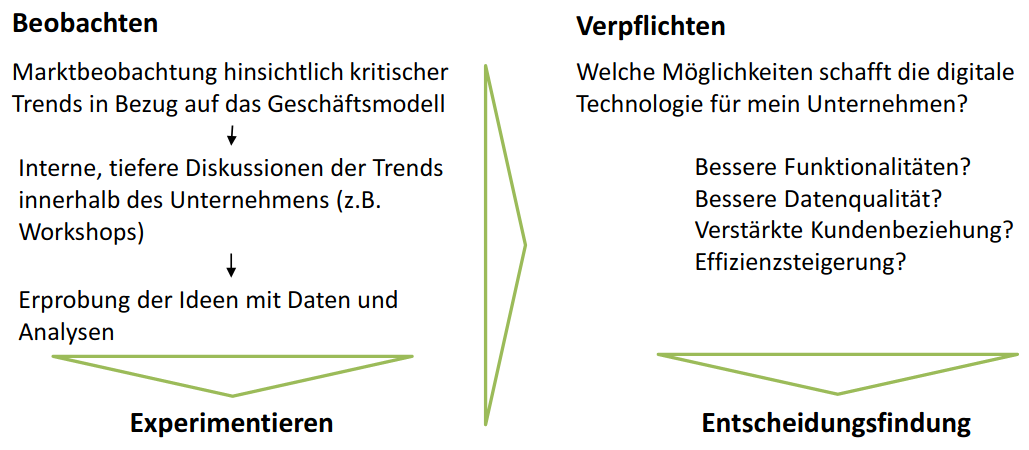
\includegraphics[scale=0.45]{experiment.png}
                  \item \emph{Black hole} vs. Optionen-orientierte Investment Strategien:
                  \item[] 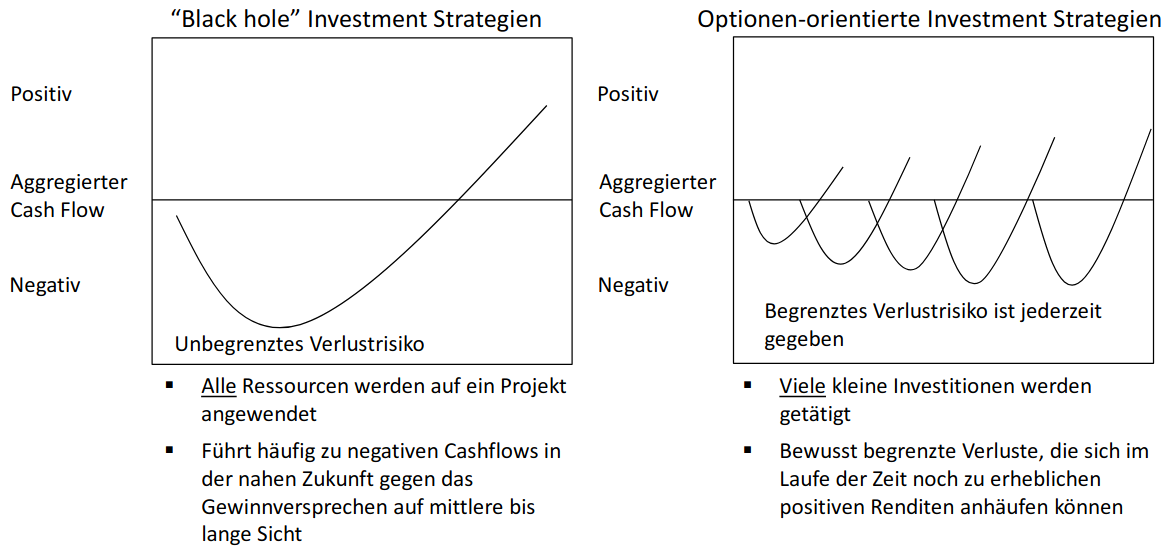
\includegraphics[scale=0.4]{bh.png}
               \end{itemize}

         \item Phase 2: Kollision im Kern (Alt/Traditionell vs. Neu/Modern)
               \begin{itemize}
                  \item Kollision von Strategien:\\
                        Aufstrebendes Start-Up vs. etabliertes Unternehmen der Branche vs. digitales Großunternehmen
                  \item Kollision der Organisation:\\
                        Effizienz-Nachteile in Durchlaufzeiten, Entscheidungsgeschwindigkeit, Führ\-ungs\-mo\-del\-le
                  \item Reaktionsebenen: Koexistenz vs. Morph\\
                        Wirksame und rechtzeitige Reaktion auf aufstrebende, digitale Konkurrenten.
                        \begin{itemize}
                           \item Ergänzung der Konkurrenten: Aufbau eines digitalen Geschäfts-modells als Koexistenz zum Konkurrenten
                           \item Morph: Ersetzen des traditionellen-durch ein digitales Geschäftsmodells
                        \end{itemize}
               \end{itemize}

         \item Phase 3: Neuerfindung an der Wurzel
               \begin{itemize}
                  \item Veränderung der Kernelemente des Geschäftsmodells durch digitale Technologien
               \end{itemize}

      \end{itemize}

   \item[] $\rightarrow$ \textbf{Architekturperspektive:}
      \begin{itemize}
         \item Geschwindigkeit  $\rightarrow$ hoher Innovationsgrad (viele Drittanbieter)
         \item Stabilität $\rightarrow$ zuverlässige Kernprozesse (enge Partner)
      \end{itemize}

   \item[] $\rightarrow$ \textbf{Führungsperspesktive:}
         \begin{itemize}
            \item[] 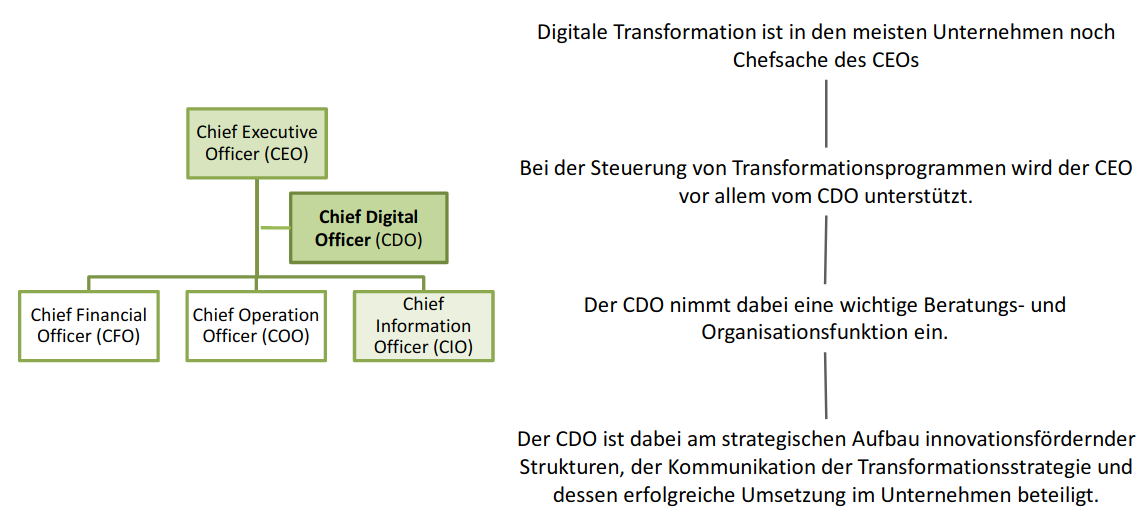
\includegraphics[scale=0.35]{ceo.png}
            \item CIO entwickelt IT-Strategie (IT-Expertenwissen)
            \item CDO legt fest (Digital-Strategisches Geschäftswissen)
            \item Unterschiede und Gemeinsamkeiten von CDO und CIO:
            \item[] 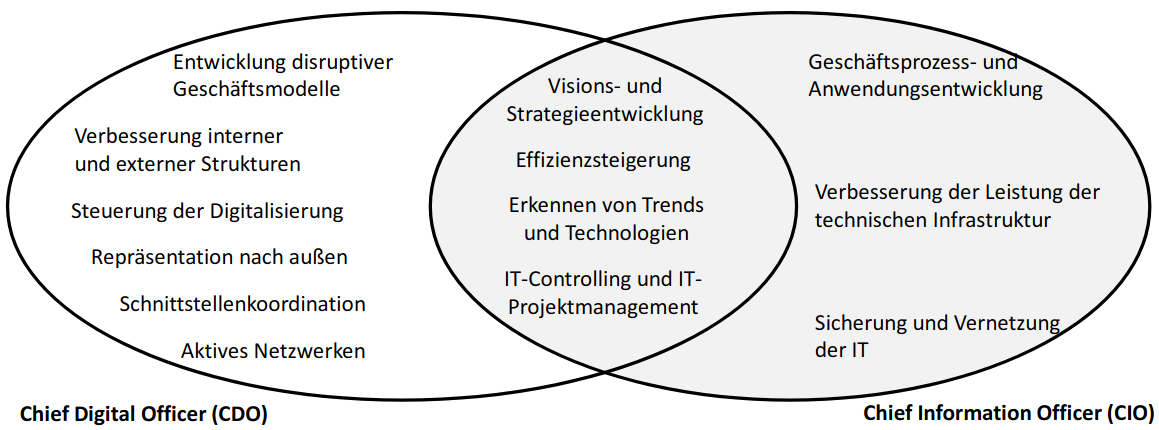
\includegraphics[scale=0.45]{ciocdo.png}
         \end{itemize}
         
\newpage %Manuelle Formatierung         
   \item \textbf{Entscheidungen einer Transformationsstrategie:}
   \item[] 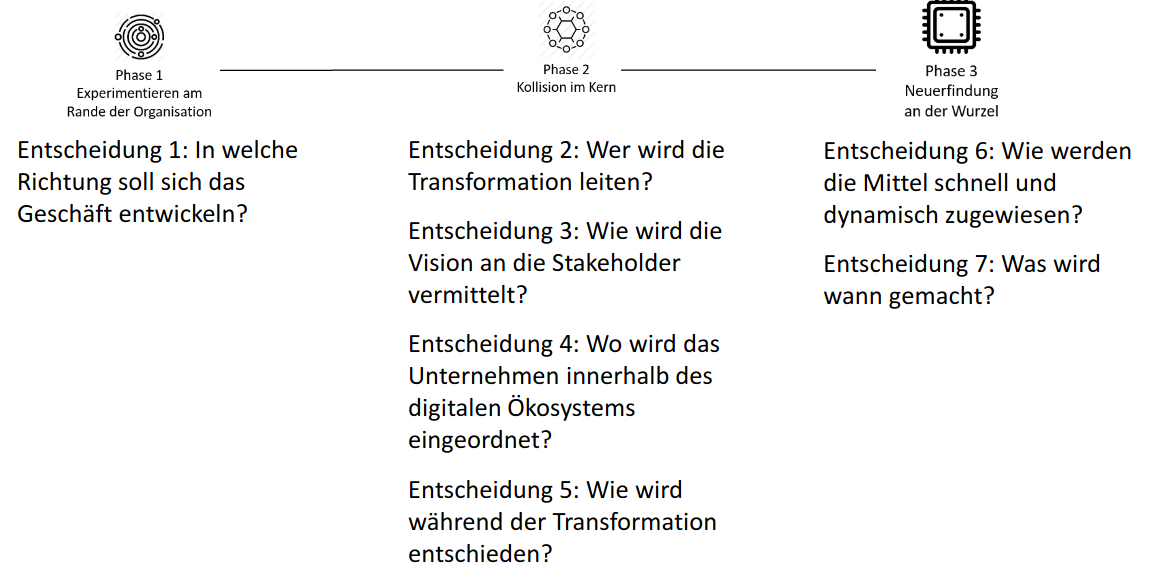
\includegraphics[scale=0.35]{dec.png}
\end{itemize}


\subsection{Voraussetzungen für die digitale Transformation schaffen} %%%%%%%%%%%%%%%%%%%%%%%%%%%%%%%%%%%%%%%%%%%%%%%%%%%%%%%%%%%%%%%%
\begin{itemize}
   \item \textbf{Die Acht Dimensionen der Digitalkultur:}
   \item[] 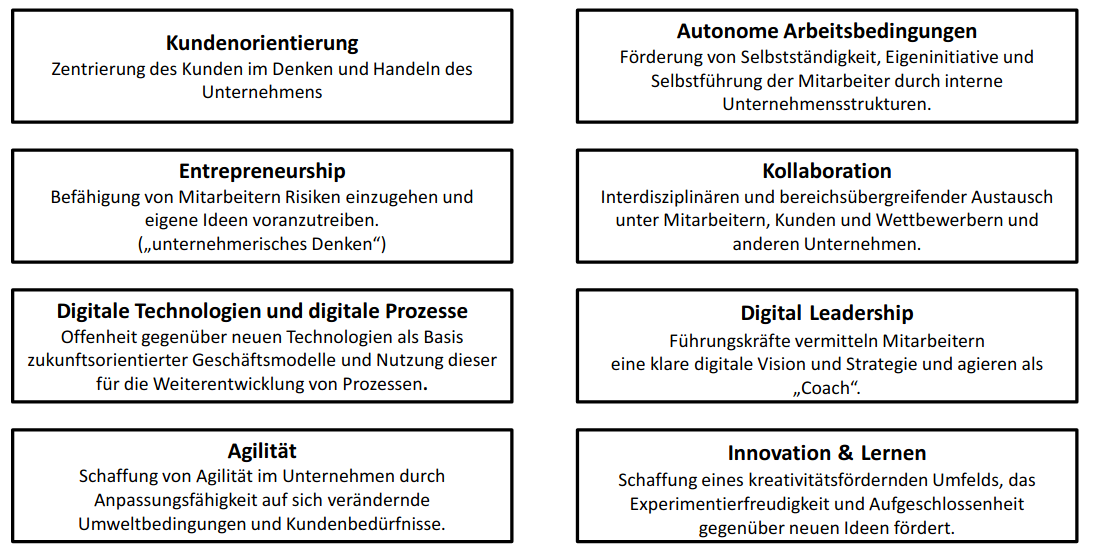
\includegraphics[scale=0.45]{8.png}
   
   \item \textbf{Transformationsfördernde OrganisationsstrukturenDigitalkultur:}
   \item[] 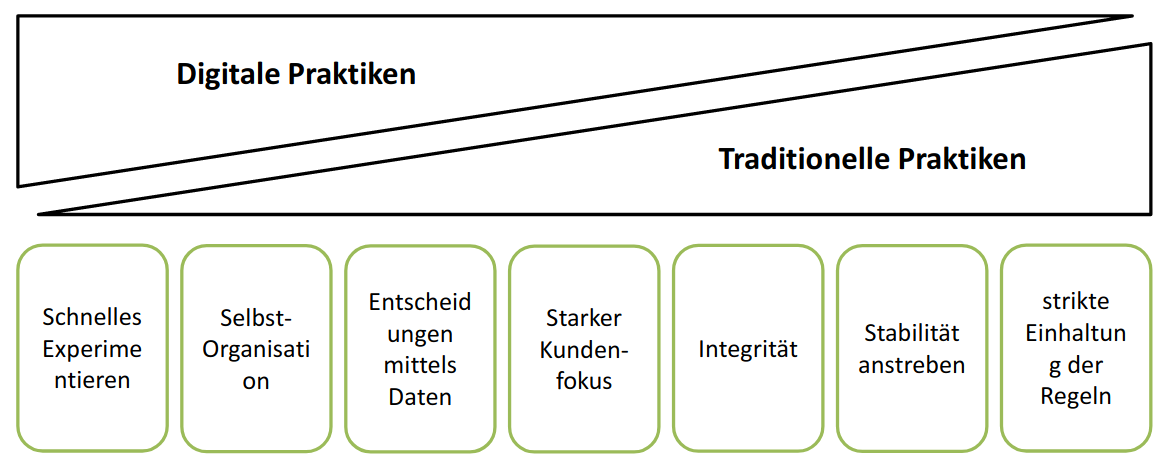
\includegraphics[scale=0.3]{altneu.png}
   
   \item \textbf{Digitale Transformation Leitfragen}
         \begin{itemize}
            \item Welche Technologien sind von zentraler Bedeutung für das Unternehmen?
            \item Mit welchen digitalen Angeboten und Prozessen werden zukünftig Erlöse generiert?
            \item Wie wird das Digitalgeschäft aufgebaut und geführt, welche strukturellen Anpassungen sind im Unternehmen erforderlich?
            \item Welche Investitionsmittel stehen zur Finanzierung des digitalen Transformationsvorhabens zur Verfügung?
         \end{itemize}

   \item \textbf{Transformationsprojekte als Enablerzur Veränderung der Organisation:}
   \item[] 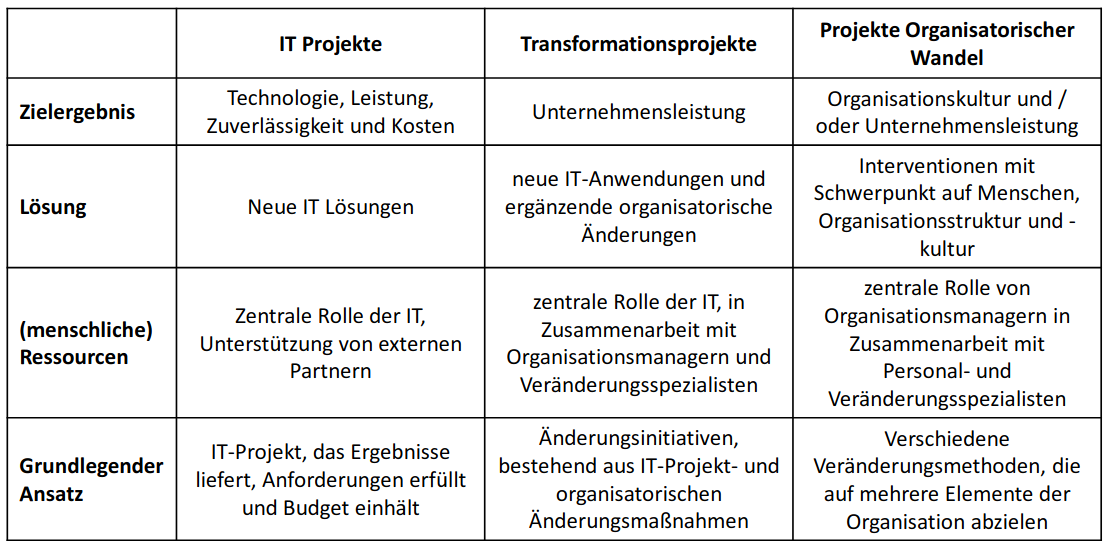
\includegraphics[scale=0.3]{ziele.png}
\end{itemize}


\vspace{0.5cm}
\subsection{QUIZFRAGEN} %%%%%%%%%%%%%%%%%%%%%%%%%%%%%%%%%%%%%%%%%%%%%%%%%%%%%%%%%%%%%%%%%%%%%%%%%%%%%%%%%%%%%%%%%%%%%%%%%%%%%%%%%%%%%%
\begin{itemize}
   \item Übernahmen aufstrebender Konkurrenten als Reaktion auf neuartige / digitale Kon\-kur\-renz können für Unternehmen eine sinnvolle Alternative darstellen.
   \item Neuartige Geschäftsmodelle fokussieren sich im wesentlichen auf die Kundenerfahrung als Kernelement ihres Geschäftsmodells
   
   \item Bei \emph{Black-Hole} Investment Strategien ist der aggregierte negative \emph{Cassh Flow} in der Regel höher als bei Optionen-orientierte Investment Strategien.
   \item Bei der Black-Hole Investment Strategie werden alle Ressourcen auf ein einzelnes Investment allokiert.
   
   \item Der CDO arbeitet in der Regel eng mit dem Chief Executive Officer (CEO) zusammen.
   \item Ein CIO kümmert sich um die Effizienzsteigerung von Unternehmensprozessen und hat die Hauptaufgabe, die IT-Infrastruktur effizient zu managen.
   \item Der CIO ist für die IT-Struktur im Unternehmen verantwortlich, waehrend der CDO hauptsaechlich für die digitales und strategische Ausrichtung verantwortlich ist.
   
   \item Eine disruptive Innovation führt häufig zu einer völligen Umstrukturierung eines Marktes durch neuartige Geschäftsmodelle.
   
   \item Das Dilemma der Innovation (\textit{Innovator's Dilemma}) beschreibt den Zustand, dass etablierte Unternehmen weiter auf ihre traditionelle Geschäftspraxis setzen und so potenziell wichtige Technologien übersehen.
         Dies kann dazu führen, dass ehemalige Marktführer aus dem Markt gedrängt werden.
         
   \item Das S-Kurven Konzept als Instrument des strategischen Innovationsmanagements besagt, dass Technologien sich im Zeitverlauf in die Entstehungsphase, die Wachstumsphase, die Reifephase sowie die Phase der Alterung einteilen lassen.
         Darüber hinaus sind Basistechnologien im Markt bereits bekannt und etabliert, sodass sie keine bzw. kaum noch Wettbewerbsvorteile mit sich bringen.
         
   \item Eine Digitalkultur befähigt Mitarbeiter unternehmerisch zu denken, um neue Ge\-schäfts\-po\-ten\-zia\-le zu erkennen.
\end{itemize}



%%%%%%%%%%%%%%%%%%%%%%%%%%%%%%%%%%%%%%%%%%%%%%%%%%%%%%%%%%%%%%%%%%%%%%%%%%%%%%%%%%%%%%%%%%%%%%%%%%%%%%%%%%%%%%%%%%%%%%%%%%%%%%%%%%%%%%
%%%% VL 6
%%%%%%%%%%%%%%%%%%%%%%%%%%%%%%%%%%%%%%%%%%%%%%%%%%%%%%%%%%%%%%%%%%%%%%%%%%%%%%%%%%%%%%%%%%%%%%%%%%%%%%%%%%%%%%%%%%%%%%%%%%%%%%%%%%%%%%
\newpage
\section{Digitale Geschäftsmodelle}

\vspace*{0.5cm}
\subsection{Digitale Güter und Märkte} %%%%%%%%%%%%%%%%%%%%%%%%%%%%%%%%%%%%%%%%%%%%%%%%%%%%%%%%%%%%%%%%%%%%%%%%%%%%%%%%%%%%%%%%%%%%%%%
\begin{itemize}
   \item \textbf{Digitales Gut:}
         \begin{itemize}
            \item Liegen in immaterieller Form vor
            \item Sind vollständig als digitale Repräsentation in Binärform gespeichert
            \item Können ohne Bindung an Trägermedium entwickelt, vertrieben oder angewendet werden (z.B. via Internet)
         \end{itemize}

   \item \textbf{Digitalisierungsgrade von Gütern:}
   \item[] 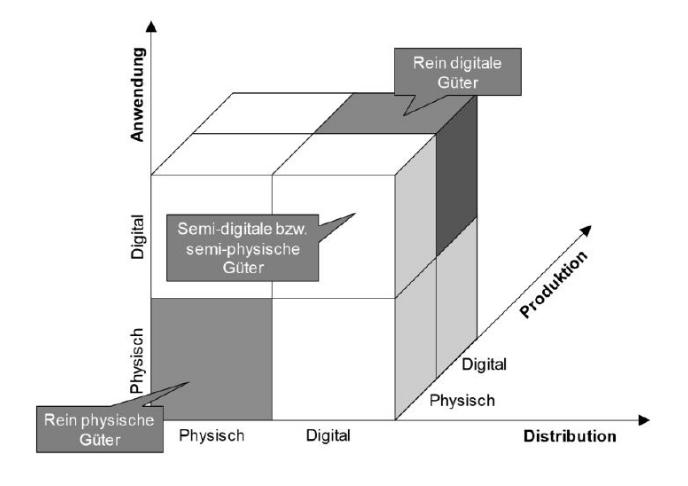
\includegraphics[scale=0.35]{wuerfel.png}
   
   \item \textbf{Eigenschaften digitaler Güter:}
         \begin{itemize}
            \item Wahrnehmungsunterschiede / Interaktivität\\
                  Digitale Güter können nur über zwei Sinne (Sehen und Hören) wahrgenommen werden.
                  Digitale Güter sind interaktiv vom Benutzer bedien- und steuerbar.
            \item Skaleneffekte\\
                  Keine Kostenvorteile entstehen bei durch sinkende Kosten pro hergestelltem Produkt.
            \item Kopierbarkeit / Verteilbarkeit\\
                  Digitale Güter werden bei Weitergabe vermehrt, nicht aufgeteilt.
            \item Veränderbarkeit / Editierbarkeit / Reprogrammierbarkeit\\
                  Digitale Güter können ohne großen Aufwand in Produktvarianten überführt und angeboten werden.
            \item Abnutzbarkeit\\
                  Digitale Güter unterliegen keinerlei Abnutzung; die Unterscheidung zwischen neuem und altem Gut entfällt.
         \end{itemize}

   \item \begin{minipage}[t]{0.43\textwidth}
            \textbf{Modularität} \\
            Möglichkeit der Zerlegung komplexer (Wertschöpfungs-) Systeme in separate Subsysteme, die für sich alleine funktionieren.
         \end{minipage} \begin{minipage}[t]{0.05\textwidth}
            \ \\
         \end{minipage} \begin{minipage}[t]{0.43\textwidth}
            \textbf{Granularität} \\
            Möglichkeit der Zerlegung digitaler Objekte bis in kleinste Elemente und Operationen.
         \end{minipage}

   \item \textbf{Eigenschaften digitaler Märkte:}
         \begin{itemize}
            \item Unendliche Informationsökonomie
                  \begin{itemize}
                     \item Jede Information kann in Form von Bits digitalisiert werden.
                     \item Menschen sind bereit, für Informationen zu zahlen. 
                     \item Der Preis von Informationsgütern richtet sich nach dem Verbraucherwert, nicht nach den Produktionskosten.
                     \item Beispiele von Informationen: Bücher, Datenbanken, Filme etc
                  \end{itemize}
            \item Skaleneffekte\\
                  Entwicklung und Vertrieb digitaler Güter verursachen hohe fixe, aber nur sehr geringe variable Kosten, wodurch sich extreme Skaleneffekte ergeben.
            \item Netzwerkeffekte\\
%                  \vspace*{-0.3cm}
                  \begin{minipage}[t]{0.6\textwidth}\vspace*{-0.3cm}
                     Der Nutzen aus einem Produkt für einen Konsumenten verändert sich, wenn sich die Anzahl gleicher oder komplementärer Parteien im Markt verändert.
                  \end{minipage} \begin{minipage}[t]{0.05\textwidth}\vspace*{-0.3cm}
                     $\ $\\
                  \end{minipage} \begin{minipage}[t]{0.3\textwidth}\vspace*{-0.3cm}
                     \includegraphics[scale=0.25]{network.png}
                  \end{minipage}
            \item Lock-In Effekte\\
                  Starke Kundenbindung an Produkte/Dienstleistungen durch hohe Wechselkosten oder Wechselbarrieren.
            \item Versionierung\\
                  Informationsprodukt in verschiedenen Versionen für verschiedene Marktsegmente anbieten
         \end{itemize}
\end{itemize}


\subsection{Geschäftsmodelle} %%%%%%%%%%%%%%%%%%%%%%%%%%%%%%%%%%%%%%%%%%%%%%%%%%%%%%%%%%%%%%%%%%%%%%%%%%%%%%%%%%%%%%%%%%%%%%%%%%%%%%%%
\begin{itemize}
   \item \textbf{Definition von Geschäftsmodellen:}
   \item[] 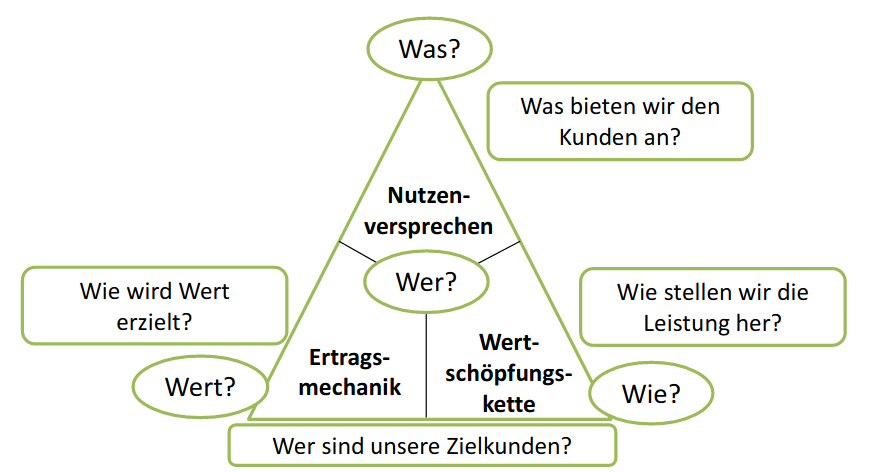
\includegraphics[scale=0.4]{wfragen.png}
   
   \newpage
   \item \textbf{Geschäftsmodelltypen:}
         \begin{itemize}
            \item \textbf{Produkt-Geschäftsmodell}
                  \begin{itemize}
                     \item standardisierte Produkte und Dienstleistungen
                     \item breite Kundenbasis
                     \item tiefe Transaktionskosten
                     \item Differenzierung durch Preis oder Leistung
                     \item Beispiel: Autos
                  \end{itemize}
            \item \textbf{Plattform-Geschäftsmodell}
                  \begin{itemize}
                     \item gemeinsame, integrative Architektur 
                     \item große Bandbreite oder Tiefe oft digitaler Angebote
                     \item Netzwerkeffekte für die Nutzer der Plattform
                     \item Differenzierung über Nutzerzahlen
                     \item Beispiel: soziale Netzwerke
                  \end{itemize}
            \item \textbf{Projekt-Geschäftsmodell}
                  \begin{itemize}
                     \item kundenindividuelle Produkte und Dienstleistungen
                     \item einmalige Leistungsvereinbarungen
                     \item Differenzierung durch Flexibilität
                     \item hoher Serviceanteil
                     \item Beispiel: Aufzug bauen
                  \end{itemize}
            \item \textbf{Lösungs-Geschäftsmodell}
                  \begin{itemize}
                     \item Kombination kundenindividueller Angebote
                     \item integrierte End-to-End Leistungen
                     \item langfristige Verträge
                     \item gegenseitige Abhängigkeit zwischen Anbieter und Abnehmer
                     \item Beispiel: Logistik
                  \end{itemize}
         \end{itemize}

   \item \textbf{Eigenschaften digitaler Geschäftsmodelle:}
   \item[] 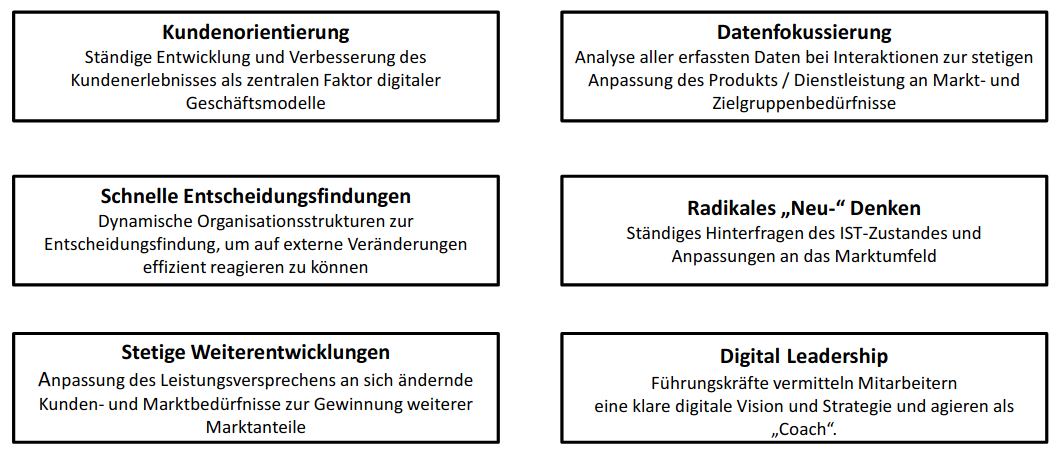
\includegraphics[scale=0.4]{edg.png}
   
   
   \newpage
   \item \textbf{Potenziale durch internen und externen Digitalisierungsfokus}
   \item[] 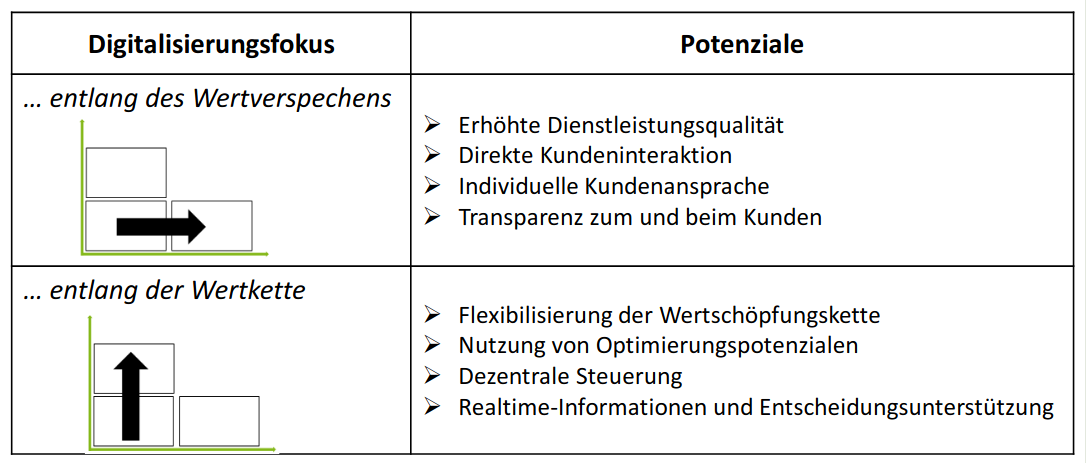
\includegraphics[scale=0.45]{potdig.png}
   
   \item \textbf{Häufige Geschäftsmodellmuster digitaler Unternehmen}
			\begin{itemize}
				\item \textbf{Freemium:}\\
						Kostenlose Basisversion und Premiumversion, oft als Abo-Modell (Dropbox)
				\item \textbf{Abonnement / Subscription:}\\
				      Nutzung der Leistung in regelmäßigen Abständen, Vertragliche Vereinbarung zwischen Kunde und Unternehmen, Zahlung in regelmäßigen Zeitabständen (Netflix)
				\item \textbf{Add-On:}\\
						Nutzen eines Services oder Produkts zu einem möglichst geringen Kaufpreis anbieten. Durch gebührenpflichtige Zusätze kann das Produkt beliebig erweitert werden (SAP)
				\item \textbf{Lock-In:}\\
						Kunden werden an ein Produkt gebunden, indem die Kosten für einen Ausstieg oder Wechsel gesteigert werden (AmazonPrime)
				\item \textbf{Rent instead of buy:}\\
						Unternehmen verkauft das Produkt nicht, sondern gewährt Kunden gegen einen kleineren Betrag zeitlich limitierte Nutzungsrechte (E-Scooter leihen)
				\item \textbf{Plattform / Mehrseitige Märkte:}\\
						Unterscheidbare Nutzergruppen, werden auf der Plattform eines Dritten zusammengeführt (Google)
			\end{itemize}
\end{itemize}


\subsection{Modellierung von Geschäftsmodellen} %%%%%%%%%%%%%%%%%%%%%%%%%%%%%%%%%%%%%%%%%%%%%%%%%%%%%%%%%%%%%%%%%%%%%%%%%%%%%%%%%%%%%%
\begin{itemize}
   \item \textbf{Ziele:}
		   \begin{itemize}
				\item Kernelemente und -logik eines Geschäftsmodells visualisieren
				\item Existierende Geschäftsmodelle besser verstehen
				\item Ideen für neue, innovative Geschäftsmodelle zu generieren
			\end{itemize}
	
	
	\newpage
	\item \textbf{Business Model Canvas (BMC):}
	      \begin{itemize}
				\item Kundennutzen (\emph{Value Proposition}) stellt Kern dar
				\item Leitfragen:
				\item[] 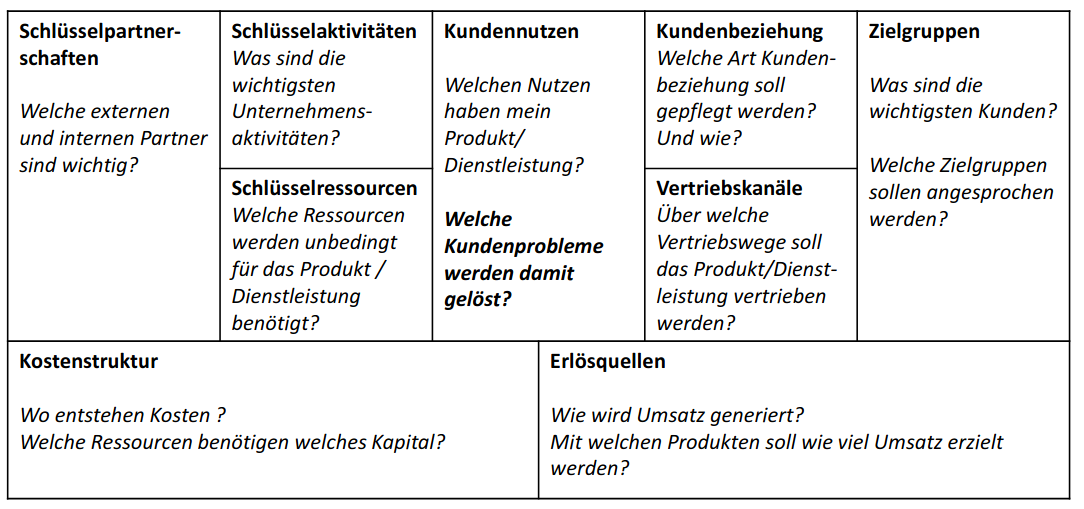
\includegraphics[scale=0.35]{BMC.png}
			\end{itemize}
	
	\item \textbf{e$^3$-Value Modellierung:}
	      \begin{itemize}
				\item Modellierungsobjekte:
				\item[] 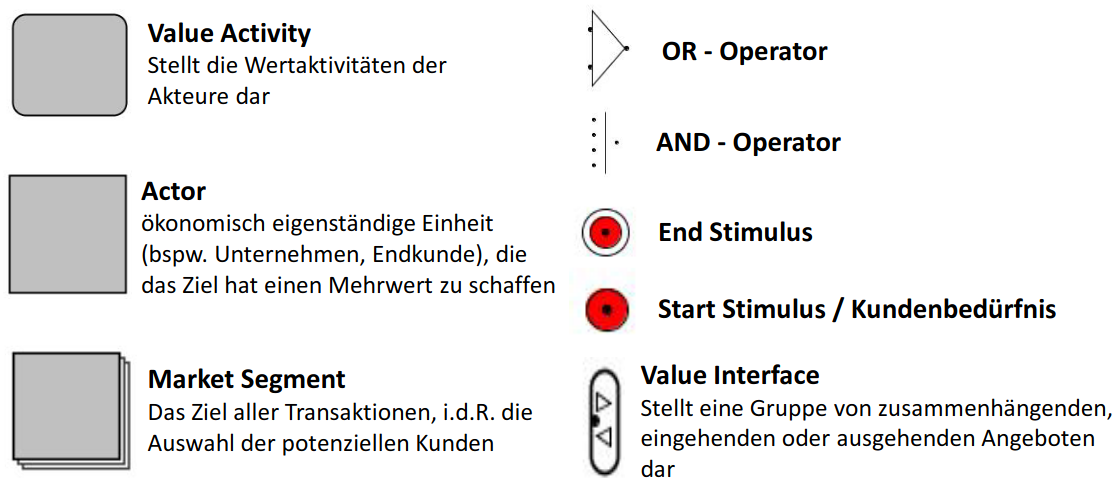
\includegraphics[scale=0.35]{modelldings.png}
				\item Beispiel eines solchen Modells:
				\item[] 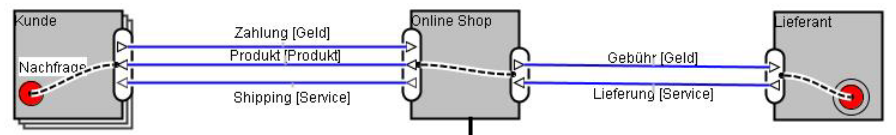
\includegraphics[scale=0.5]{beispiel_e3.png}
			\end{itemize}
	
	\item \textbf{BMC vs. e$^3$-Value:}
	\item[] \adjustbox{max width=0.9\textwidth}{%
			\begin{tabular}{r l l}
			\toprule
			    & \textbf{BMC} & \textbf{e$^3$-Value} \\
			\midrule
			\textbf{Stärken:} & ganzes Geschäftsmodell wird beschrieben & Schnittstellen werden dargestellt \\
			 & deutliche Herausstellung der Value Proposition\footnotemark & Berechnung des Wertflusses \\
			 & & Nutzenanalysen pro Akteur möglich \\
			 & &  \\
			\textbf{ Schwächen:} & keine Darstellung d. Interaktion von Akteuren & Datenbasis muss vorhanden sein \\
			 & fehlender Detaillierungsgrad & Hohe Komplexität bei größeren Netzwerken \\
			 & fehlende Nutzungsbeurteilung & keine Herausstellung der Value Proposition \\
			  & &  \\
			\textbf{Innovationsgrad:} & bei radikalen Innovationen sinnvoll & bei inkrementellen\footnotemark \ Innovationen sinnvoll \\
			\bottomrule
			\end{tabular}}
\end{itemize}

\footnotetext[4]{Nutzenversprechen (englisch value proposition) beschreibt, welchen Nutzen ein Unternehmen seinen Kunden mit einem bestimmten Produkt oder einer bestimmten Dienstleistung verspricht. }

\footnotetext[5]{Bei inkrementeller Innovation werden bekannte Technologien, Produkte, Dienstleistungen, Geschäftsmodelle oder Prozesse weiterentwickelt, bleiben aber im Kern erhalten.}


\vspace{0.5cm}
\subsection{QUIZFRAGEN} %%%%%%%%%%%%%%%%%%%%%%%%%%%%%%%%%%%%%%%%%%%%%%%%%%%%%%%%%%%%%%%%%%%%%%%%%%%%%%%%%%%%%%%%%%%%%%%%%%%%%%%%%%%%%%
\begin{itemize}
   \item Rein digitale Geschäftsmodelle basieren auf der Sammlung von Informationen und der Verarbeitung dieser.
   \item Digitale Güter lassen sich erschwert vergleichen und es herrscht eine Informationssymmetrie zwischen Preis und Qualität.
   \item Im Gegensatz zu nicht-digitalen Gütern besteht kein Unterschied zwischen dem Original und einer Kopie.
         Eine Duplizierung bei digitalen Gütern ist einfacher als bei nicht-digitalen Gütern.
   \item Die Skaleneffekte digitaler Güter ermöglichen hohe Marktanteile durch die Fixkostendegression.
   \item Anwendungssoftware oder \textit{Cloud-Comuting} Dienstleistungen sind \emph{keine} rein digitalen Güter.
   
   \item Für die \textit{e3-Value}-Methode sind sinnvolle Daten essentiell, um den vollen Nutzen zu generieren.
   \item Die \textit{e3-Value}-Methode benötigt eine hohe Datenintegration um sinnvolle Ergebnisse zu liefern.
   \item Anders als das BMC (\textit{Business Model Canvas}) ist eine umfassende Wirtschaftlichkeitsanalyse bei der \textit{e3-Value}-Methode möglich.
   \item Das BMC (\textit{Business Model Canvas}) sollte in der frühen Innovationsphase angewendet werden, da es einen guten Überblick über das ganzheitliche Geschäftsmodell liefert.
         Es stellt den Kundennutzen sehr deutlich heraus.
   \item Die Modellierung eines Geschäftsmodells kann \emph{nicht} verwendet werden, um Konkurrenten im Markt detailliert zu analyisieren.
   
   \item Auf dem digitalen Markt ist der Lock-in-Effekt ein Mittel der Netzwerkanbieter, um Kunden stärker an sich zu binden.
         Durch starke Skaleneffekte können Monopole entstehen.
   \item Auf elektronischen Märkten können sich $n$ Nachfrager und $m$ Anbieter in einer $n:m$-Beziehung gegenüberstehen.
   \item Die Markttransparenz auf elektronischen Märkten ist als hoch einzustufen.
\end{itemize}



%%%%%%%%%%%%%%%%%%%%%%%%%%%%%%%%%%%%%%%%%%%%%%%%%%%%%%%%%%%%%%%%%%%%%%%%%%%%%%%%%%%%%%%%%%%%%%%%%%%%%%%%%%%%%%%%%%%%%%%%%%%%%%%%%%%%%%
%%%% VL 7
%%%%%%%%%%%%%%%%%%%%%%%%%%%%%%%%%%%%%%%%%%%%%%%%%%%%%%%%%%%%%%%%%%%%%%%%%%%%%%%%%%%%%%%%%%%%%%%%%%%%%%%%%%%%%%%%%%%%%%%%%%%%%%%%%%%%%%
\newpage
\section{Geschäftsmodellinnovation und digitale Plattformen}

\vspace*{0.5cm}
\subsection{Digitale Technologien und Geschäftsmodellinnovation} %%%%%%%%%%%%%%%%%%%%%%%%%%%%%%%%%%%%%%%%%%%%%%%%%%%%%%%%%%%%%%%%%%%%%
\begin{itemize}
   \item \textbf{Geschäftsmodellinnovation:}\\
         Verändern sich mindestens zwei Dimensionen eines Geschäftsmodells signifikant, spricht man von einer Geschäftsmodellinnovation.

   \item \textbf{Vergleich traditioneller und neuartiger, digitaler Wirtschaft:}
   \item[] 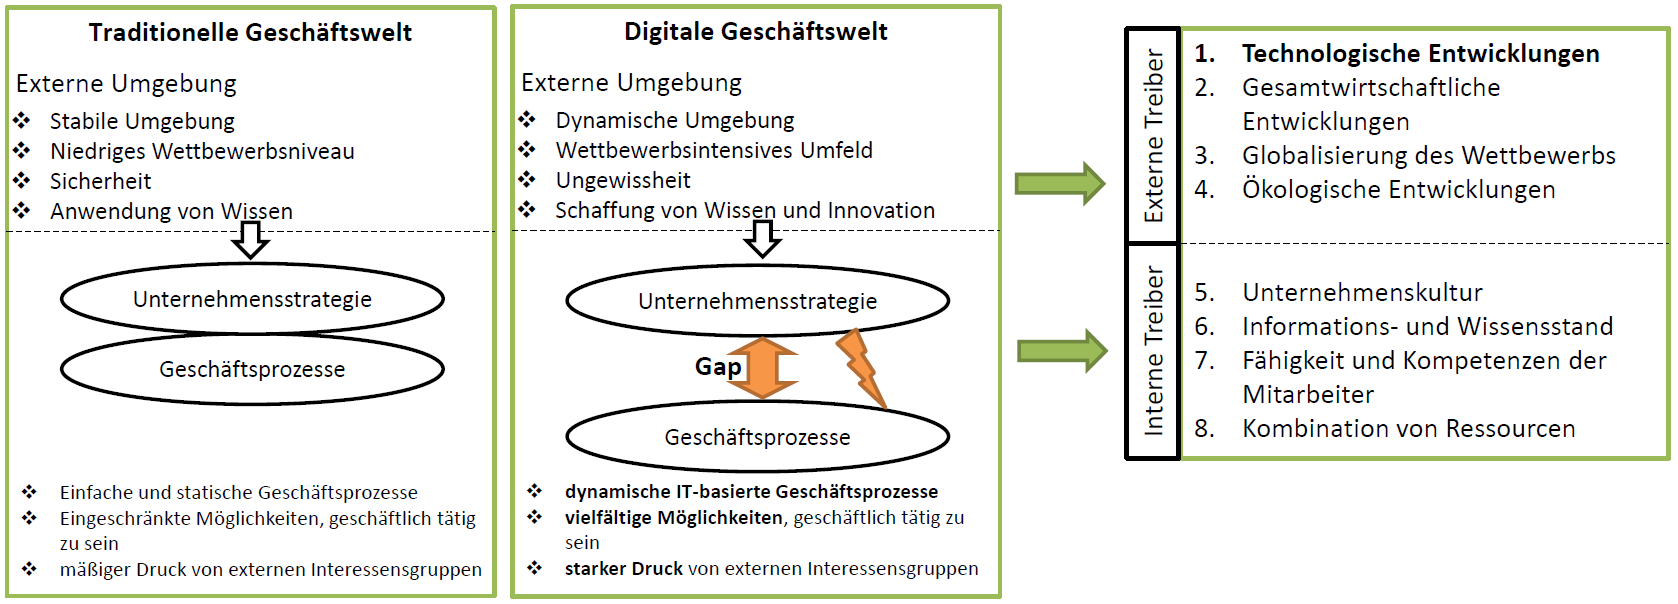
\includegraphics[scale=0.35]{TraditionellVsDigital.png}
   
   \item \textbf{Innovationsgrade der Geschäftsinnovation:} \vspace*{-0.5cm}
   \item[] \begin{minipage}[t]{0.35\textwidth} \vspace*{0cm}
               \begin{itemize}
		            \item \textbf{Radikale Innovation:}\\
		                  Fundamentale Veränderungen in angrenzenden oder neuen Märkten (Hohes Chancen–Risiko Verhältnis)
		            \item \textbf{Inkrementelle Innovation:}\\
		                  Geringfügige Veränderungen, die etablierte Produkt-Markt-Felder fortführen (Geringes Chancen–Risiko Verhältnis)
		         \end{itemize}
            \end{minipage} \begin{minipage}[t]{0.05\textwidth} \vspace*{0cm}
               $\ $ \\
            \end{minipage} \begin{minipage}[t]{0.5\textwidth} \vspace*{0cm}
               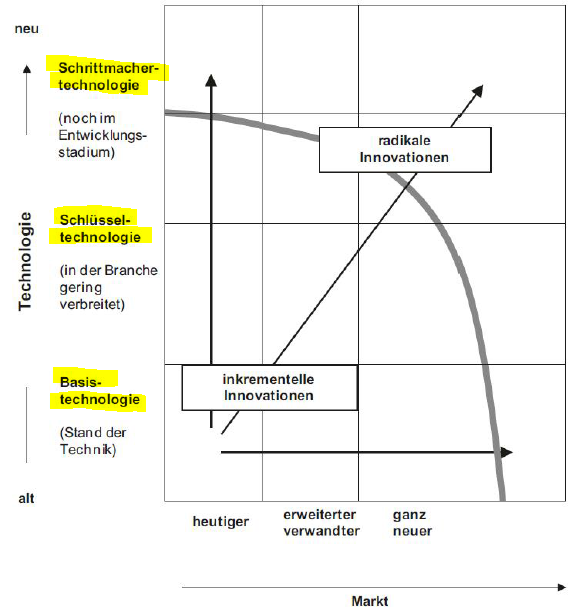
\includegraphics[scale=0.55]{InnovationsgradeH.png}
            \end{minipage}
   
   \newpage
   \item \textbf{Potenziale digitaler Technologien für Geschäftsmodellinnovation:}
         \begin{itemize}
            \item ($\uparrow$) Weniger gebundene Innovationen
            \item ($\rightarrow$) Weniger Grenzen zwischen Innovationsprozess und -ergebnissen
            \item ($\leftarrow$) Mehr Innovationsakteure
         \end{itemize}

   \item \textbf{Werttreiber digitaler Geschäftsmodelle:}
         \begin{itemize}
            \item \textbf{Novelty} (Neuigkeitsgehalt):\\
                  Wie soll das bestehendes Geschäftsmodell verändert werden und sich somit von der Konkurrenz abgrenzen?
            \item \textbf{Lock-In} (Kunden-/ Lieferantenbindung):\\
                  Wie können wir Kunden und Partner an das Geschäftsmodell binden?
            \item \textbf{Complementarities} (Komplementaritäten):\\
                  Wo lassen sich Synergien mit bestehenden Kompetenzen schaffen?
            \item \textbf{Efficiencies} (Effizienz):\\
                  In wie fern ist die neue Architektur günstiger und/oder liefert einen höheren Wert für den Kunden?
         \end{itemize}
   
   \item \textbf{Drei zentrale Komponenten eines digitalen Geschäftsmodells:}
   \item[] 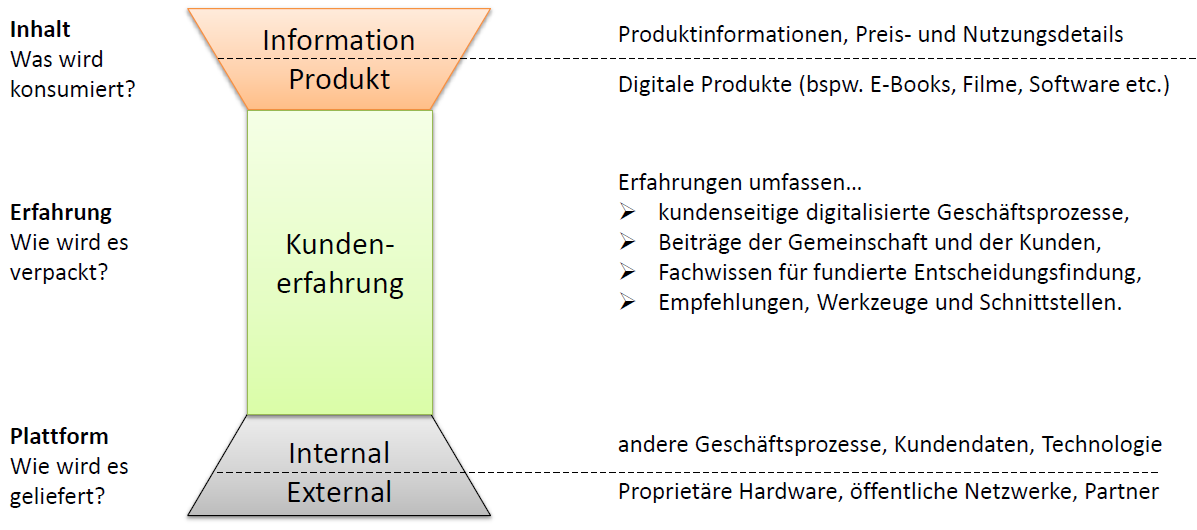
\includegraphics[scale=0.47]{DreiKomponenten.png}
\end{itemize}


\subsection{Digitale Plattformen} %%%%%%%%%%%%%%%%%%%%%%%%%%%%%%%%%%%%%%%%%%%%%%%%%%%%%%%%%%%%%%%%%%%%%%%%%%%%%%%%%%%%%%%%%%%%%%%%%%%%
\begin{itemize}
   \item \textbf{Prinzip:}\\
         Eine Plattform basiert darauf wertschöpfende Interaktionen zwischen externen Produzenten und Konsumenten zu ermöglichen.
   
   
   \newpage
   \item \textbf{Vier Kernelemente digitaler Plattformen:}
   \item[] 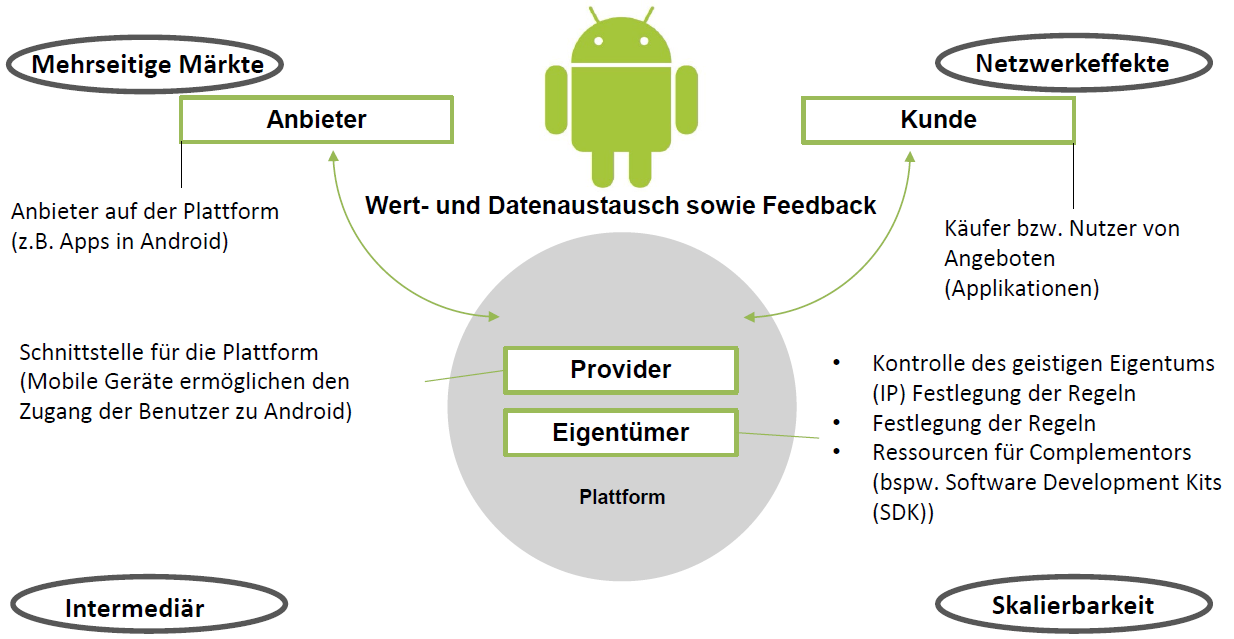
\includegraphics[scale=0.42]{VierKernelemente.png}
   
   \item \textbf{Eigenschaften einer digitalen Plattform:}
         \begin{itemize}
            \item Ist ein Nexus aus Regeln und Architektur
            \item Ist offen, erlaubt geregelte Teilnahme
            \item Fördert aktiv (positive) Interaktionen zwischen verschiedenen Partnern in einem mehrseitigen Markt
            \item Skaliert viel schneller als ein Pipeline-Geschäft, weil es nicht zwingend die Kosten der externen Produktion trägt
         \end{itemize}
   
   \item \textbf{Netzwerkeffekte digitaler Plattformen:}
         \begin{itemize}
            \item \textbf{Direkte Netzwerkeffekte:}\\
                  Mehr Nutzer eines Produkts oder Services führen zu größerem Nutzen für alle Mitglieder des Netzwerkes.
            \item \textbf{Indirekte Netzwerkeffekte:}\\
                  Mehr Nutzer eines Produkts oder Services erhöhen den Wert von Komplementärprodukten auf der Plattform.Mehr Komplementärprodukte machen die Plattform attraktiver für Nutzer.
         \end{itemize}
   
   \item \textbf{Architektur digitaler Plattformen $–$ Sozio-technische Perspektive:}
   \item[] 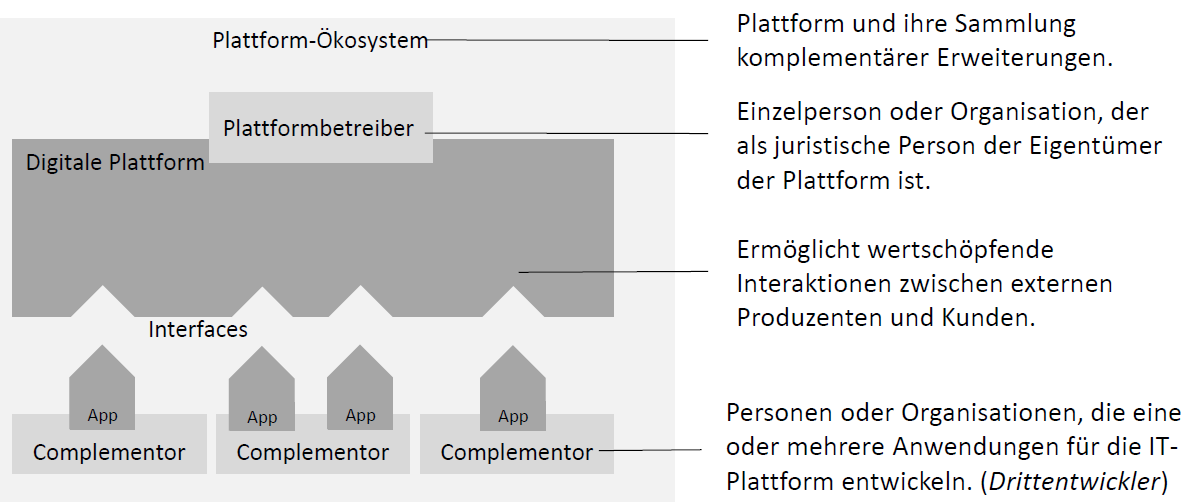
\includegraphics[scale=0.43]{ArchitekturDigitalerPlattformen.png}
   \item[] Die Bereitstellung von API \textit{Application Programming Interfaces} (im Bereich der \textit{Interfaces}) durch den Plattformbesitzer zur Anbindung von Applikationen in die Plattform ermöglicht:
         \begin{itemize}
            \item Möglichkeit der Zusammenarbeit mit externen Akteuren
            \item Reduzierung von Integrationskomplexität
            \item Möglichkeit der offenen Innovation
            \item Erhöhung der Reichweite und Präsenz am Markt
         \end{itemize}
   
   \item \textbf{Charakteristika digitaler Plattformen:}
         \begin{itemize}
            \item \textbf{Henne-Ei Problematik:}\\
                  Das Henne-Ei-Problem beschreibt die Herausforderung, Nutzer einer Marktseite für die Plattform zu gewinnen, bevor eine kritische Masse an anderen Nutzern einer anderen Marktseite präsent ist.
            \item \textbf{Multi Homing:}\\
                  Multihoming beschreibt den parallelen Einsatz mehrerer Plattformen auf einer der Nutzerseiten.
                  Plattformbetreiber wollen Multihoming vermeiden, um Wettbewerbsvorteile zu erzielen (z.B. durch exklusive Inhalte).
            \item \textbf{Winner-takes-it-all:}\\
                  Winner-takes-it-all-Effekte entstehen dadurch, dass sich durch die selbst\-ver\-stärk\-en\-den Wachstumseffekte meist ein dominierender Anbieter durchsetzt, der die konkurrierenden Betreiber in eine Nische oder ganz vom Markt verdrängt.
         \end{itemize}
\end{itemize}


\vspace{0.5cm}
\subsection{QUIZFRAGEN} %%%%%%%%%%%%%%%%%%%%%%%%%%%%%%%%%%%%%%%%%%%%%%%%%%%%%%%%%%%%%%%%%%%%%%%%%%%%%%%%%%%%%%%%%%%%%%%%%%%%%%%%%%%%%%
\begin{itemize}
   \item Für die Plattform \emph{Ebay} bestehen Indirekte Netzwerkeffekte zwischen Käufer und Händler.
   
   \item In der digitalen Geschäftswelt sind vornehmlich dynamische IT-basierte Ge\-schäfts\-mo\-del\-le zu finden und durch die dynamische Umgebung in der digitalen Geschäftswelt kommt es zu verstärktem Wettbewerbsdruck.
   
   \item Plattformbetreiber stellen häufig Schnittstellen für Drittparteien zu Verfügung, was die Reichweite und Präsenz am Markt erhöht, es Drittentwickler ermöglicht die Innovationskraft der Plattform zu steigern und die Integrationskomplexität reduziert.
   
   \item Die Henne-Ei Problematik beschreibt im Allgemeinen die Schwierigkeit verschiedene Parteien als Nutzer der Plattform zu gewinnen.
         Sie besagt, dass Vielfältige, selbst\-ver\-stärk\-en\-de Effekte (Netzwerkeffekte) erst generiert werden können, sobald die kritische Masse erreicht wurde
   
   \item Bei digitalen Plattformen führen Skaleneffekte und Netzwerkeffekte maßgeblich zur Marktkonzentration (Winner-takes-it-all).
   
   \item Der Lock-In Effekte bei digitalen Plattformen kann Vertragsbindungen und Netzwerkeffekte begünstigen.
   
   \item Externe Einflussfaktoren können einen Einfluss auf die Geschäftsmodellinnovation ausüben.
   \item Mit der Digitalisierung verlagert sich der Schwerpunkt von einzelnen Innovationsakteuren auf sich entwickelnde Innovationskollektive mit unterschiedlichen Zielen, Motiven und Fähigkeiten.
   \item Mit der Digitalisierung gibt es weniger Grenzen und eine komplexere, dynamischere Interaktion zwischen Innovationsprozessen und -ergebnissen.
   
   \item Digitale Plattformen haben die Eigenschaften Intermediär und Zweiseitige Märkte.
\end{itemize}
\end{document}






